\begin{apendicesenv}

\partapendices


\chapter{Testes ALPR}\label{teste_alpr}
\begin{lstlisting}[basicstyle=\scriptsize, caption=Resultado de saída em JSON de testes com a \textit{Fn-ALPR}]
{
  "status_code": 200,
  "response": {
    "uuid": "ccad04ec-7896-45be-a91d-fff2e645d55e",
    "data_type": "alpr_results",
    "epoch_time": 1559258933552,
    "processing_time": {
      "plates": 472.6234130859375,
      "total": 540.9680000011576
    },
    "img_height": 1080,
    "img_width": 1920,
    "results": [
      {
        "plate": "AYZ6152",
        "confidence": 90.21435546875,
        "region_confidence": 78,
        "vehicle_region": {
          "y": 457,
          "x": 641,
          "height": 451,
          "width": 451
        },
        "region": "br-sp",
        "plate_index": 0,
        "processing_time_ms": 39.33467102050781,
        "candidates": [
          {
            "matches_template": 1,
            "plate": "AYZ6152",
            "confidence": 90.21435546875
          },
          {
            "matches_template": 0,
            "plate": "AY6152",
            "confidence": 79.2620620727539
          },
          {
            "matches_template": 1,
            "plate": "AYX6152",
            "confidence": 78.17359161376953
          },
          {
            "matches_template": 1,
            "plate": "AYA6152",
            "confidence": 77.68161010742188
          },
          {
            "matches_template": 1,
            "plate": "AYR6152",
            "confidence": 77.67607879638672
          },
          {
            "matches_template": 0,
            "plate": "AZ6152",
            "confidence": 77.66014862060547
          },
          {
            "matches_template": 1,
            "plate": "AYJ6152",
            "confidence": 77.65591430664062
          },
          {
            "matches_template": 1,
            "plate": "AYP6152",
            "confidence": 77.64949798583984
          },
          {
            "matches_template": 1,
            "plate": "AYV6152",
            "confidence": 77.64859008789062
          },
          {
            "matches_template": 1,
            "plate": "AYT6152",
            "confidence": 77.64820098876953
          }
        ],
        "coordinates": [
          {
            "y": 735,
            "x": 813
          },
          {
            "y": 741,
            "x": 924
          },
          {
            "y": 780,
            "x": 922
          },
          {
            "y": 775,
            "x": 810
          }
        ],
        "matches_template": 1,
        "requested_topn": 10
      }
    ],
    "version": 2,
    "error": false,
    "regions_of_interest": [
      {
        "y": 0,
        "x": 0,
        "height": 1080,
        "width": 1920
      }
    ]
  }
}
\end{lstlisting}

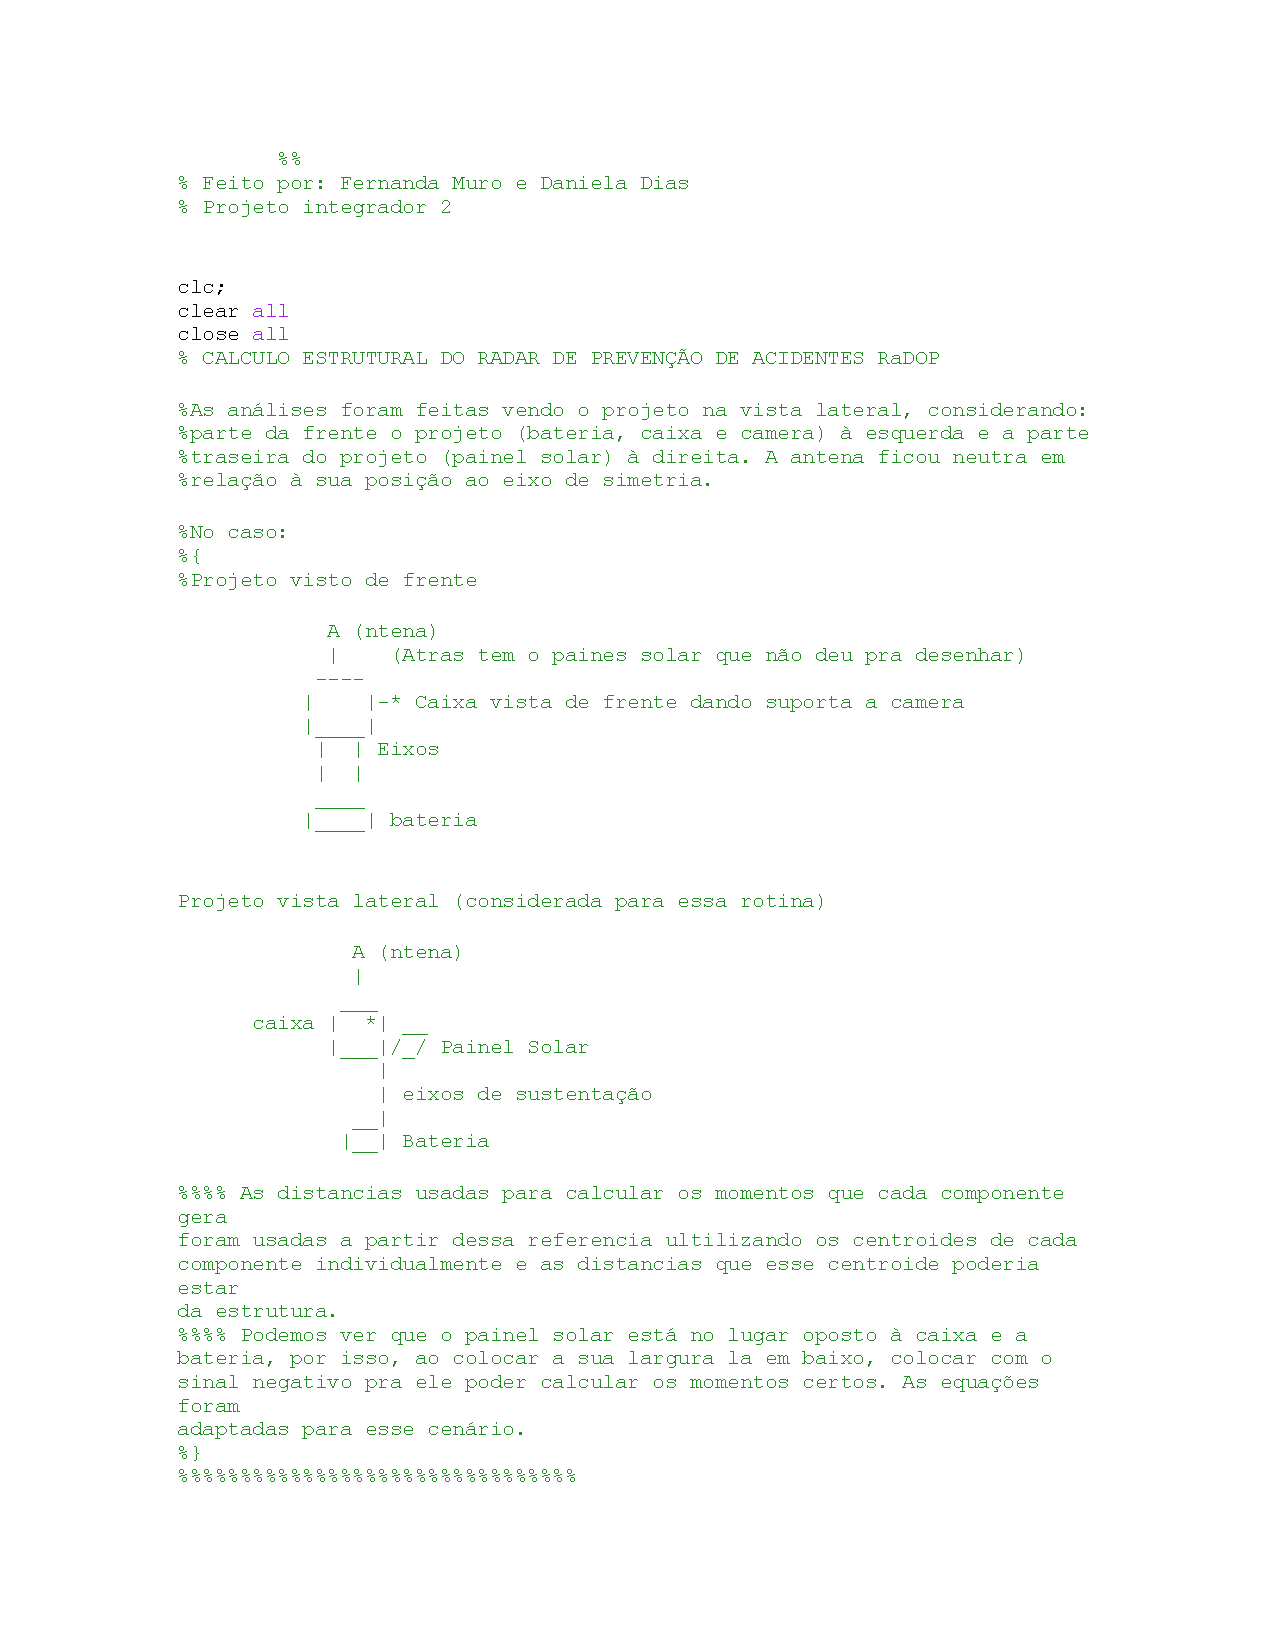
\includepdf[pages={1},scale=0.75,pagecommand= \chapter{Códigos da Estrutura Estática}\label{codigo_estatico}]{estatico.pdf}
\includepdf[pages={2-},scale=0.8,pagecommand= {}]{estatico.pdf}
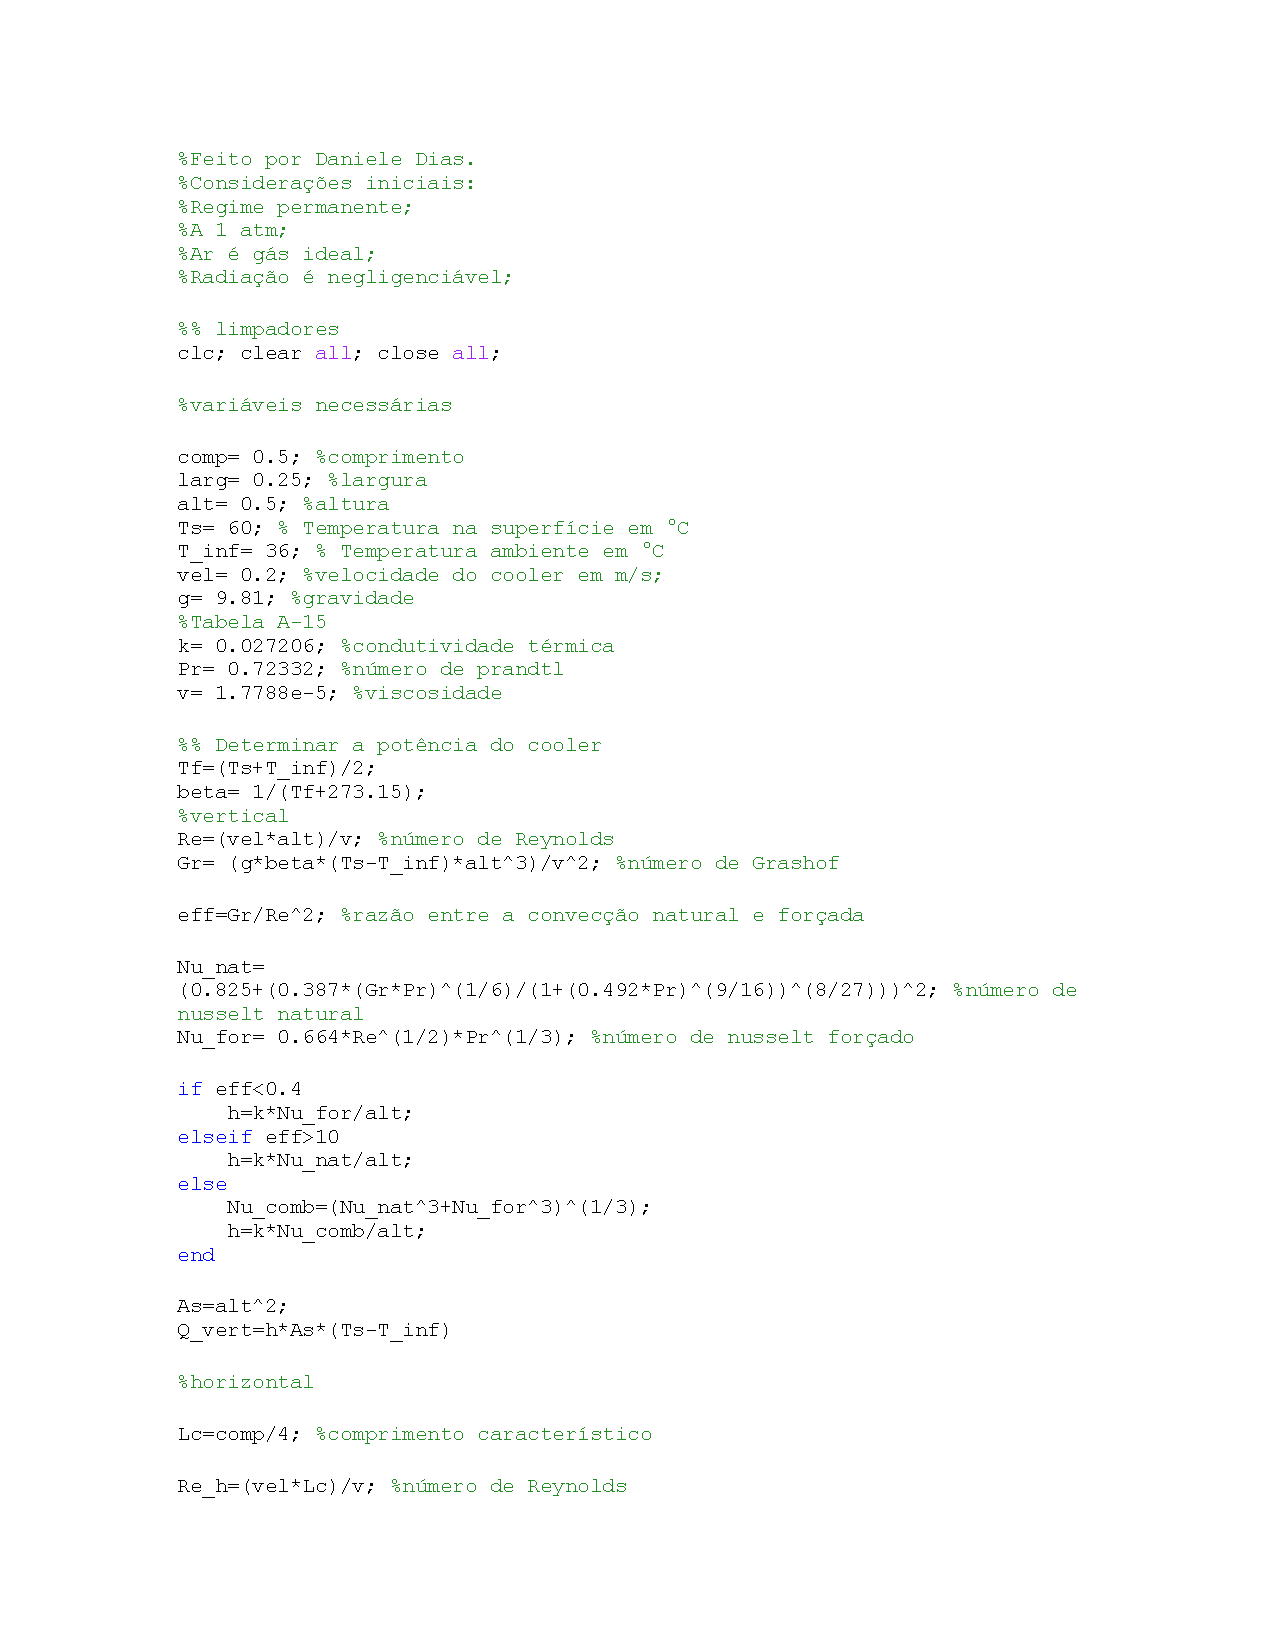
\includepdf[pages={1},scale=0.75,pagecommand= \chapter{Código para a dissipação de calor}\label{codigo_dissipacao}]{dissipacao.pdf}
\includepdf[pages={2},scale=0.8,pagecommand= {}]{dissipacao.pdf}
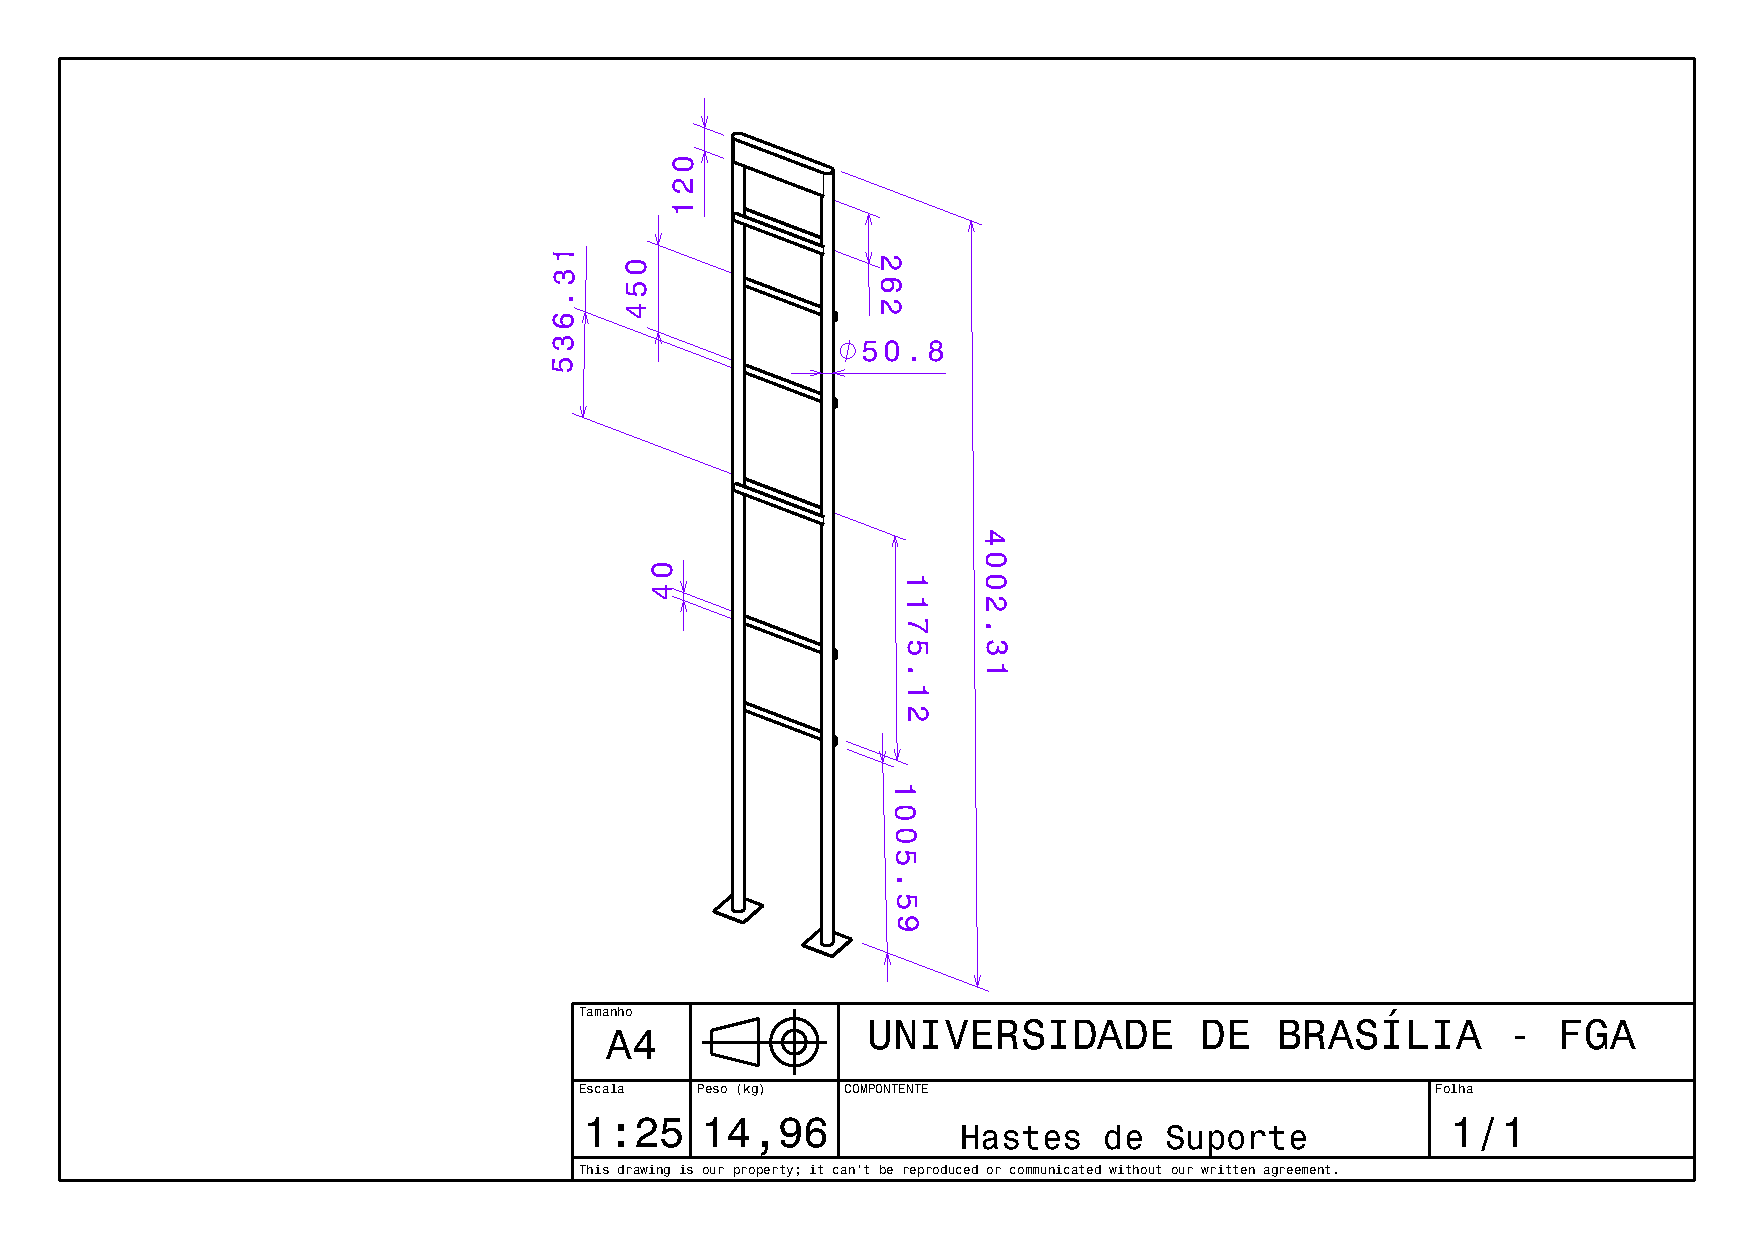
\includepdf[angle=90,scale=0.65, pagecommand= \chapter{Desenhos Técnicos apresentados}\label{plantas_construcao}]{Haste.pdf}
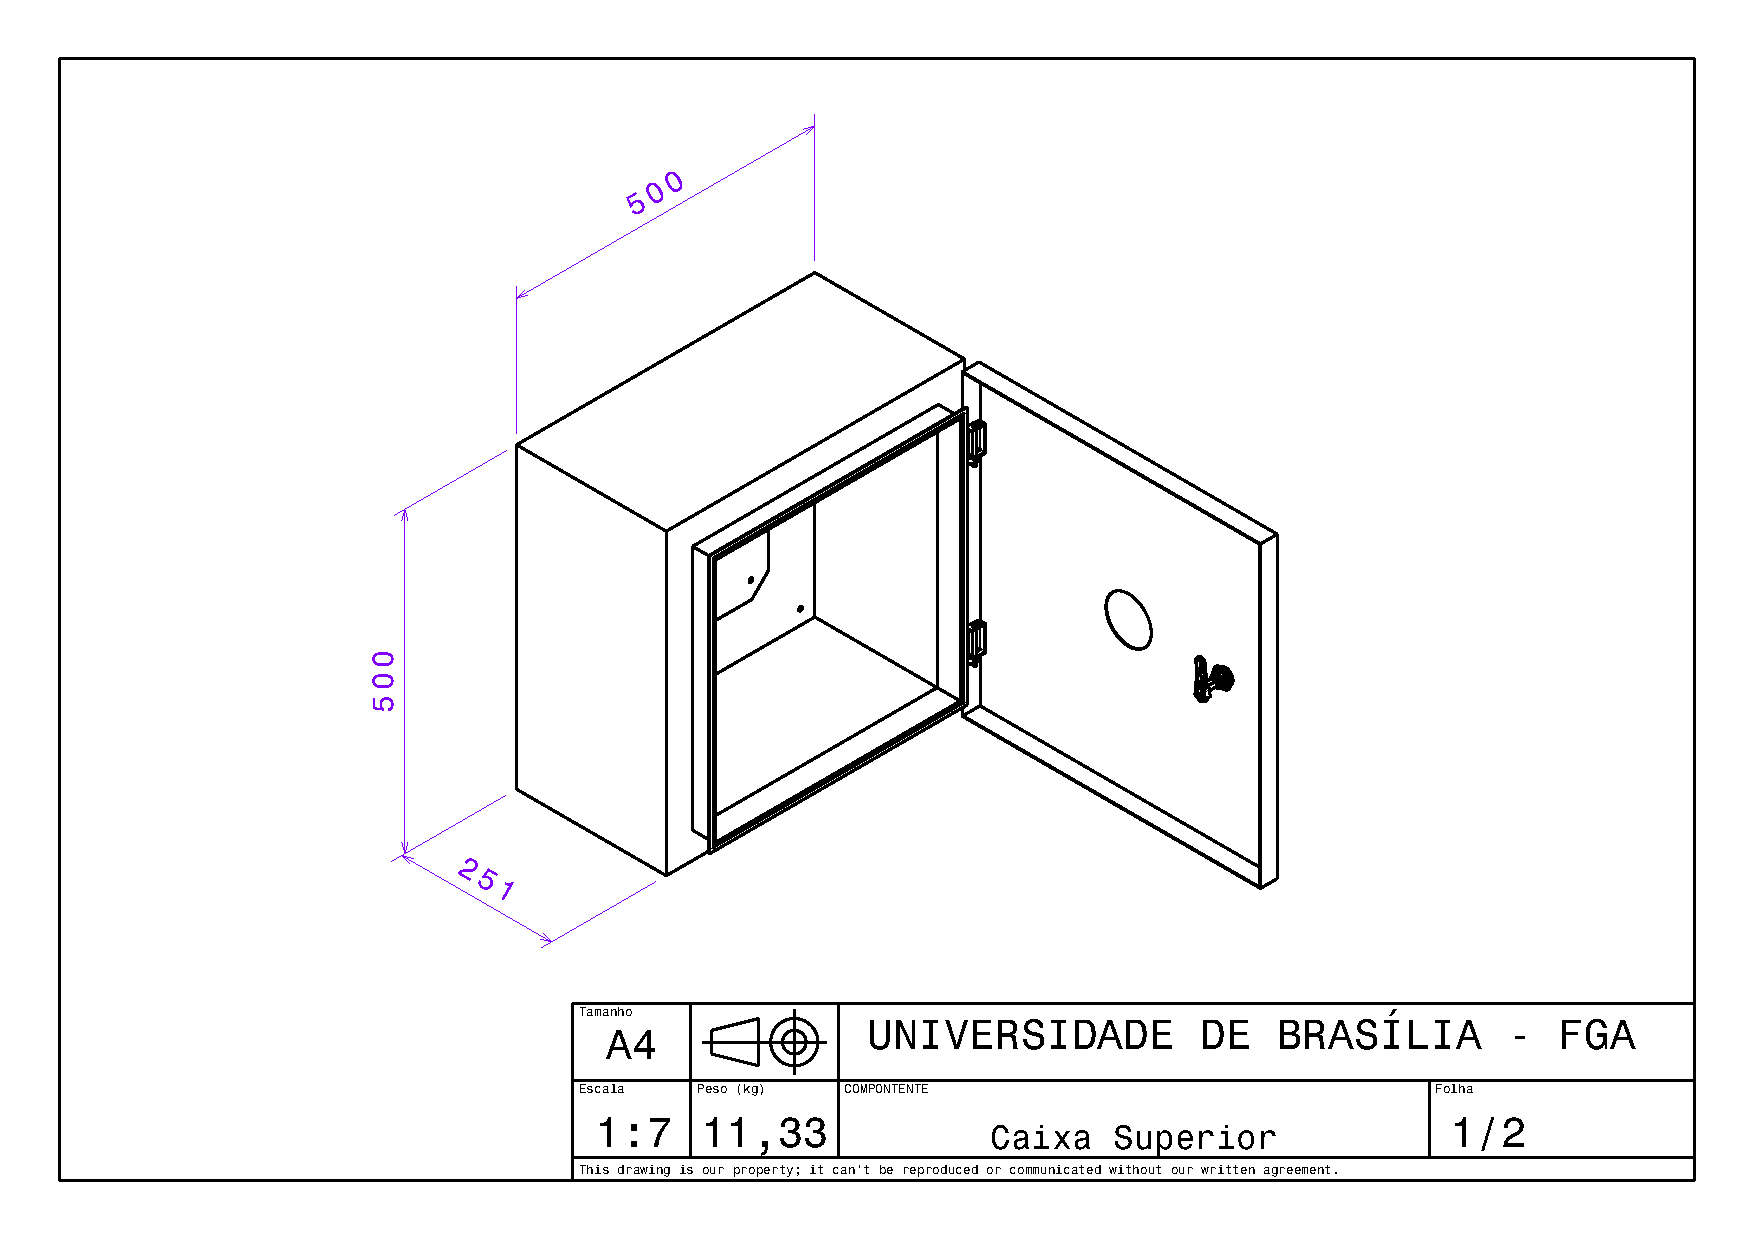
\includepdf[angle=90, scale=0.75]{CaixaSup1.pdf}
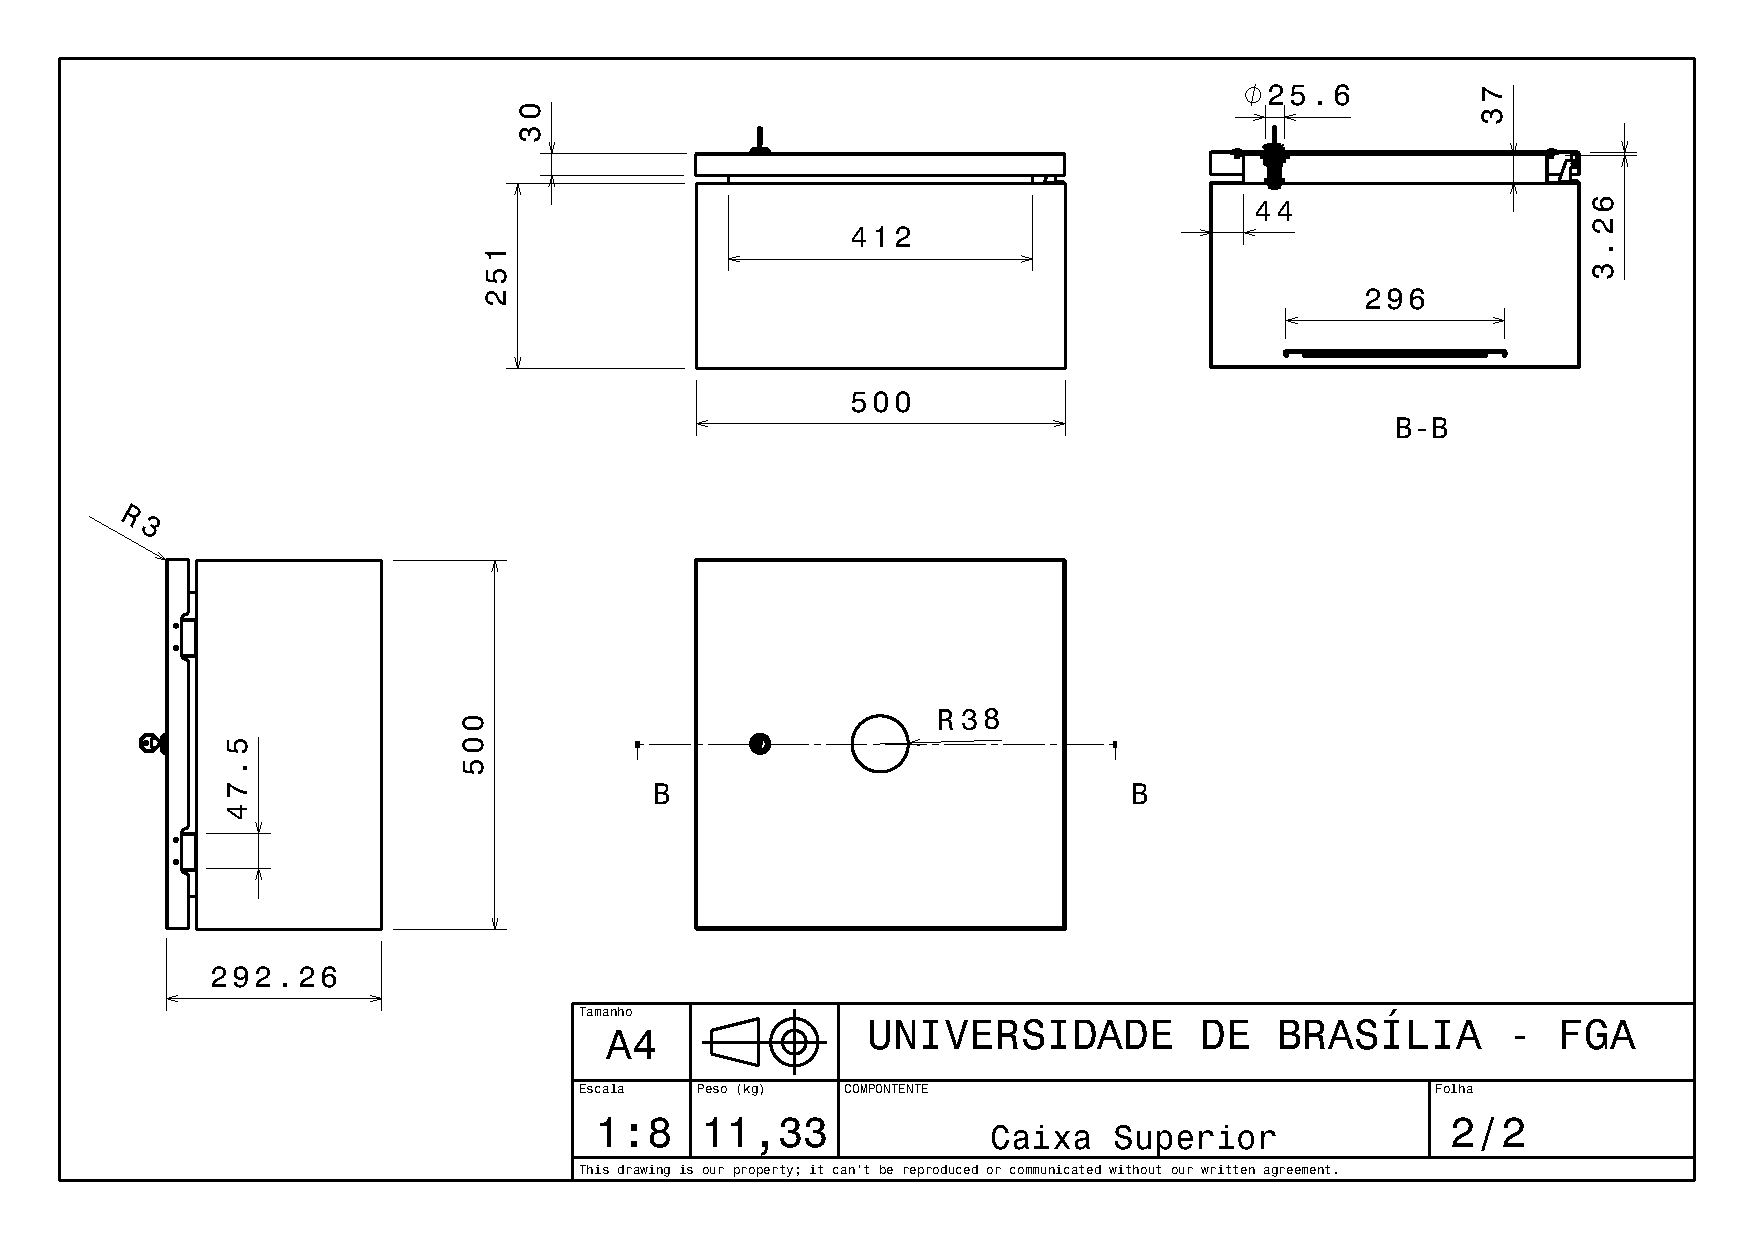
\includepdf[angle=90, scale=0.75]{CaixaSup2.pdf}
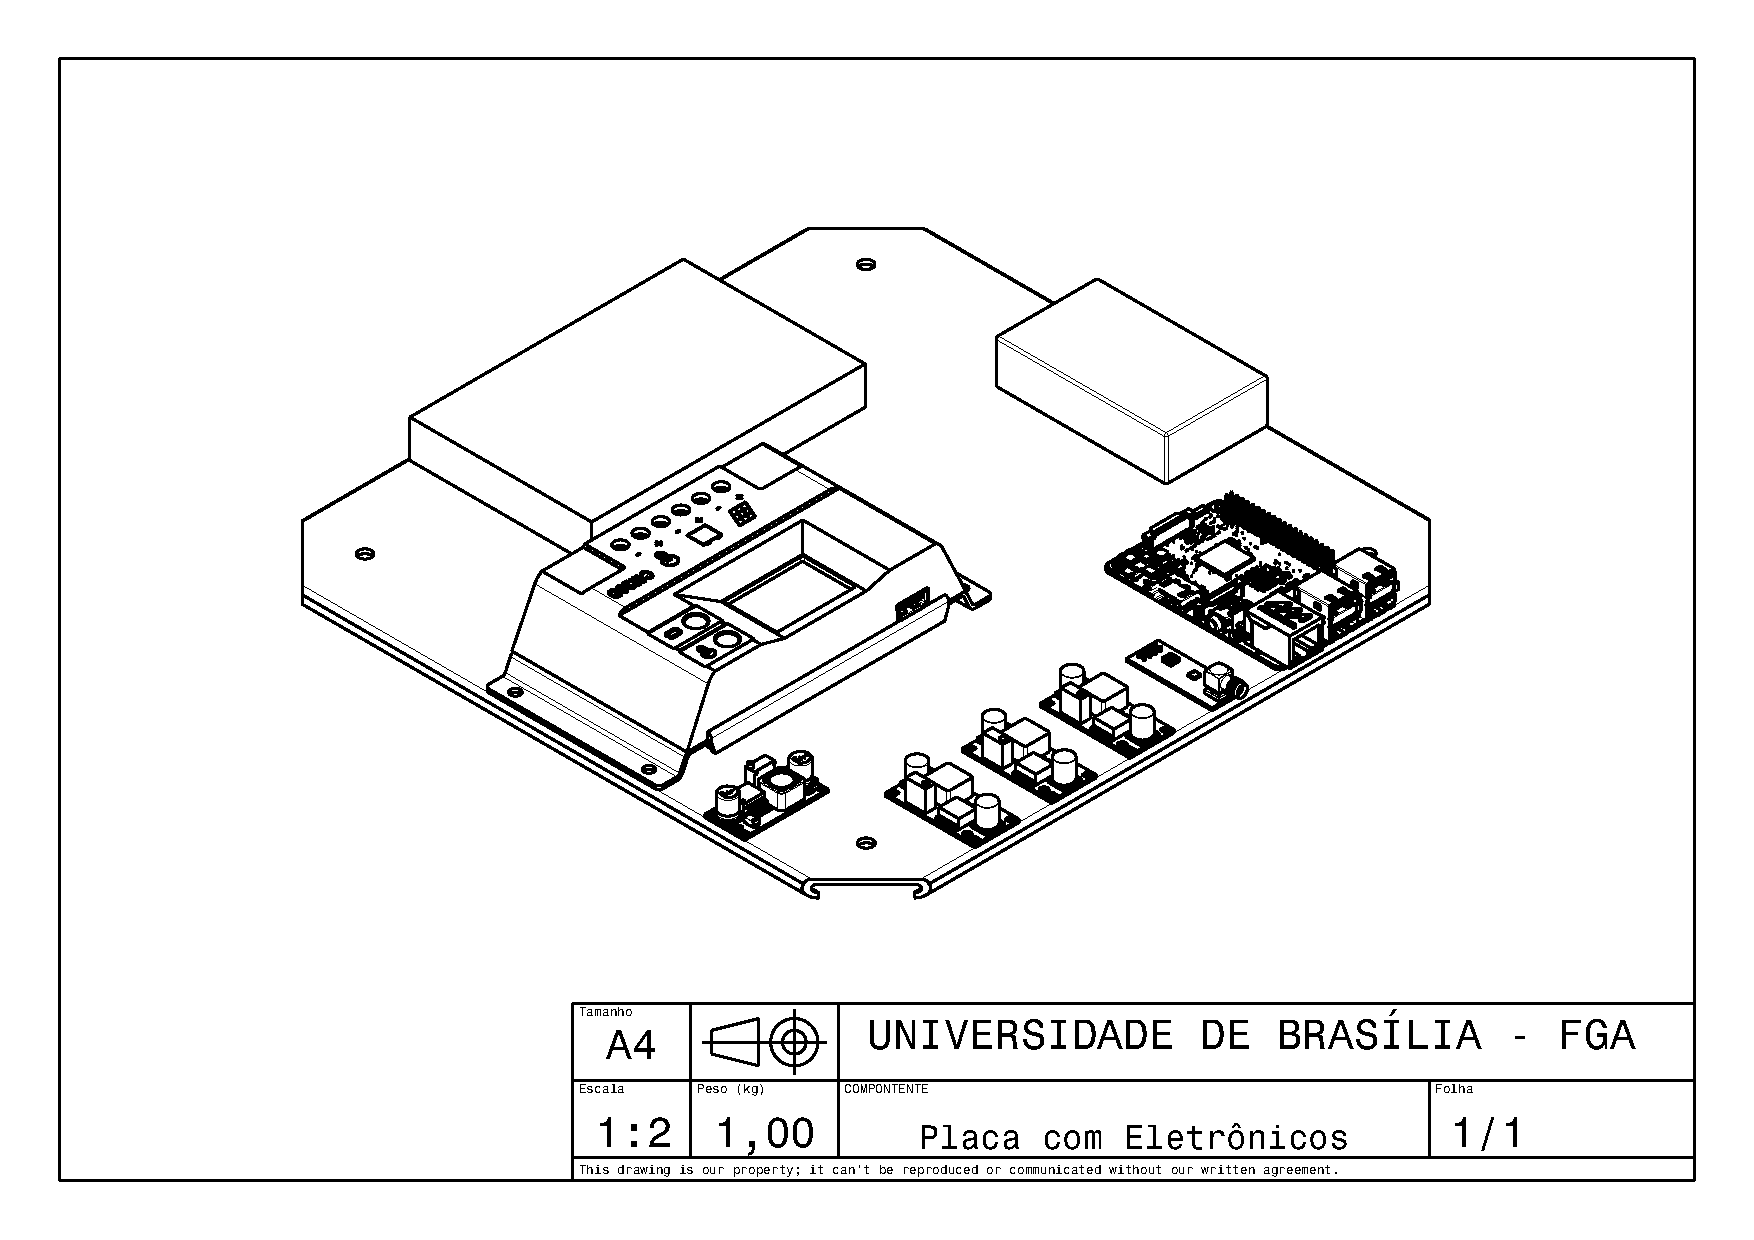
\includepdf[angle=90, scale=0.75]{Eletronicos.pdf}
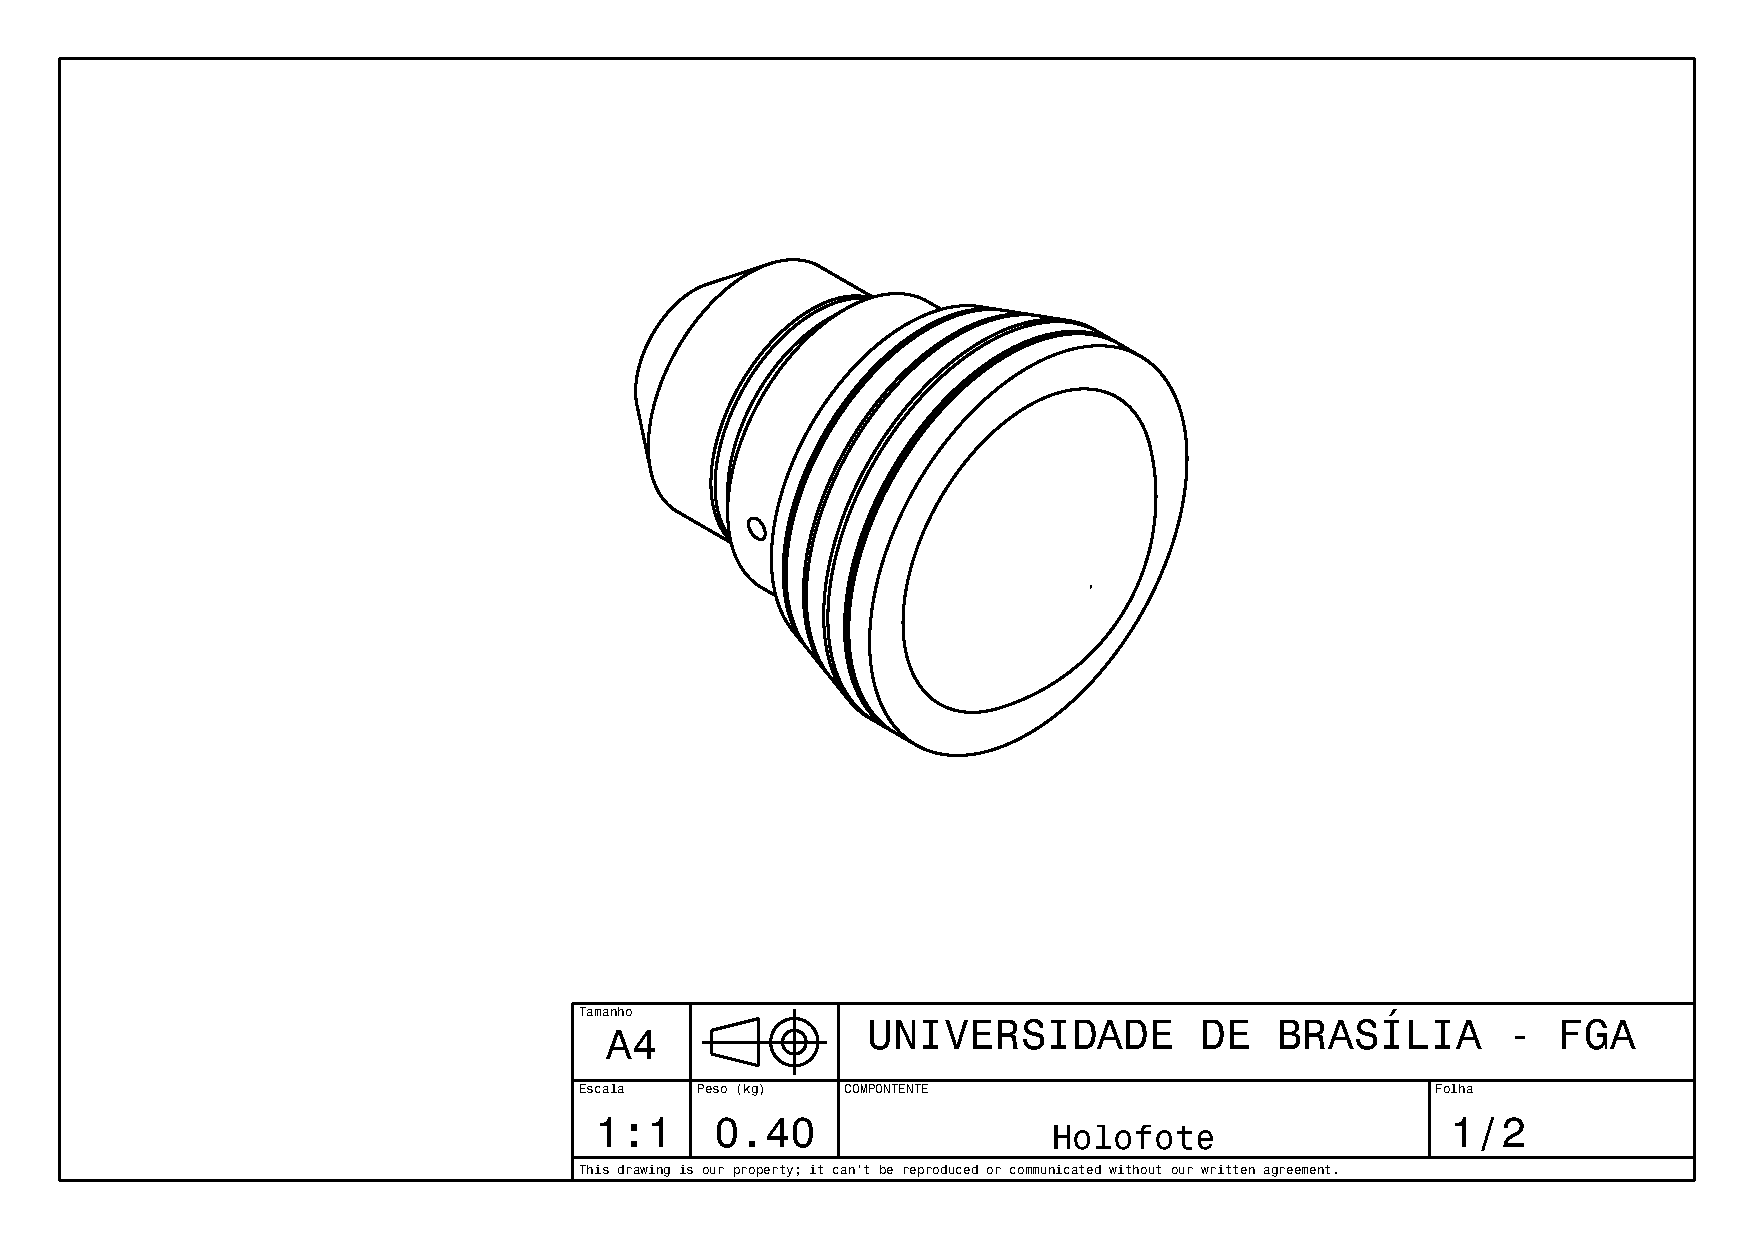
\includepdf[angle=90, scale=0.75]{Holofote1.pdf}
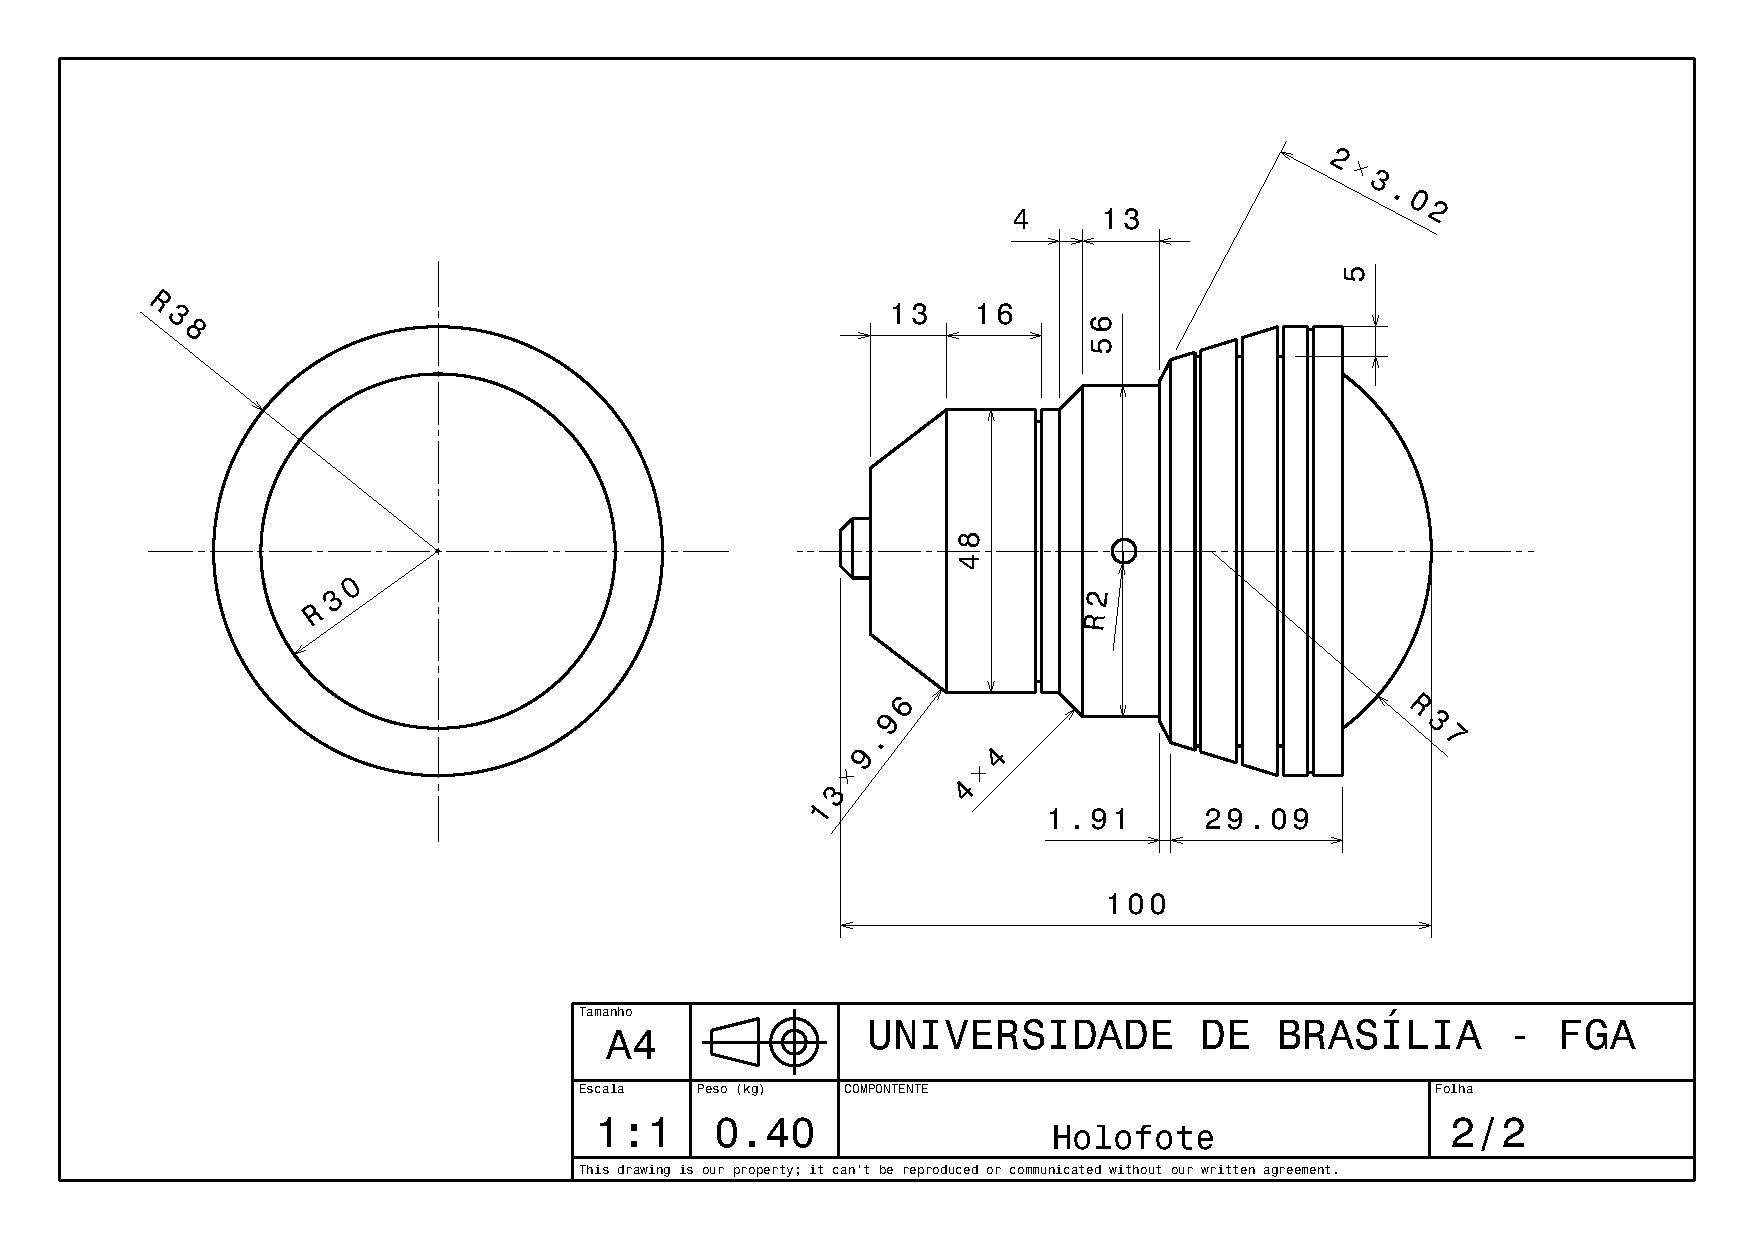
\includepdf[angle=90, scale=0.75]{Holofote2.pdf}
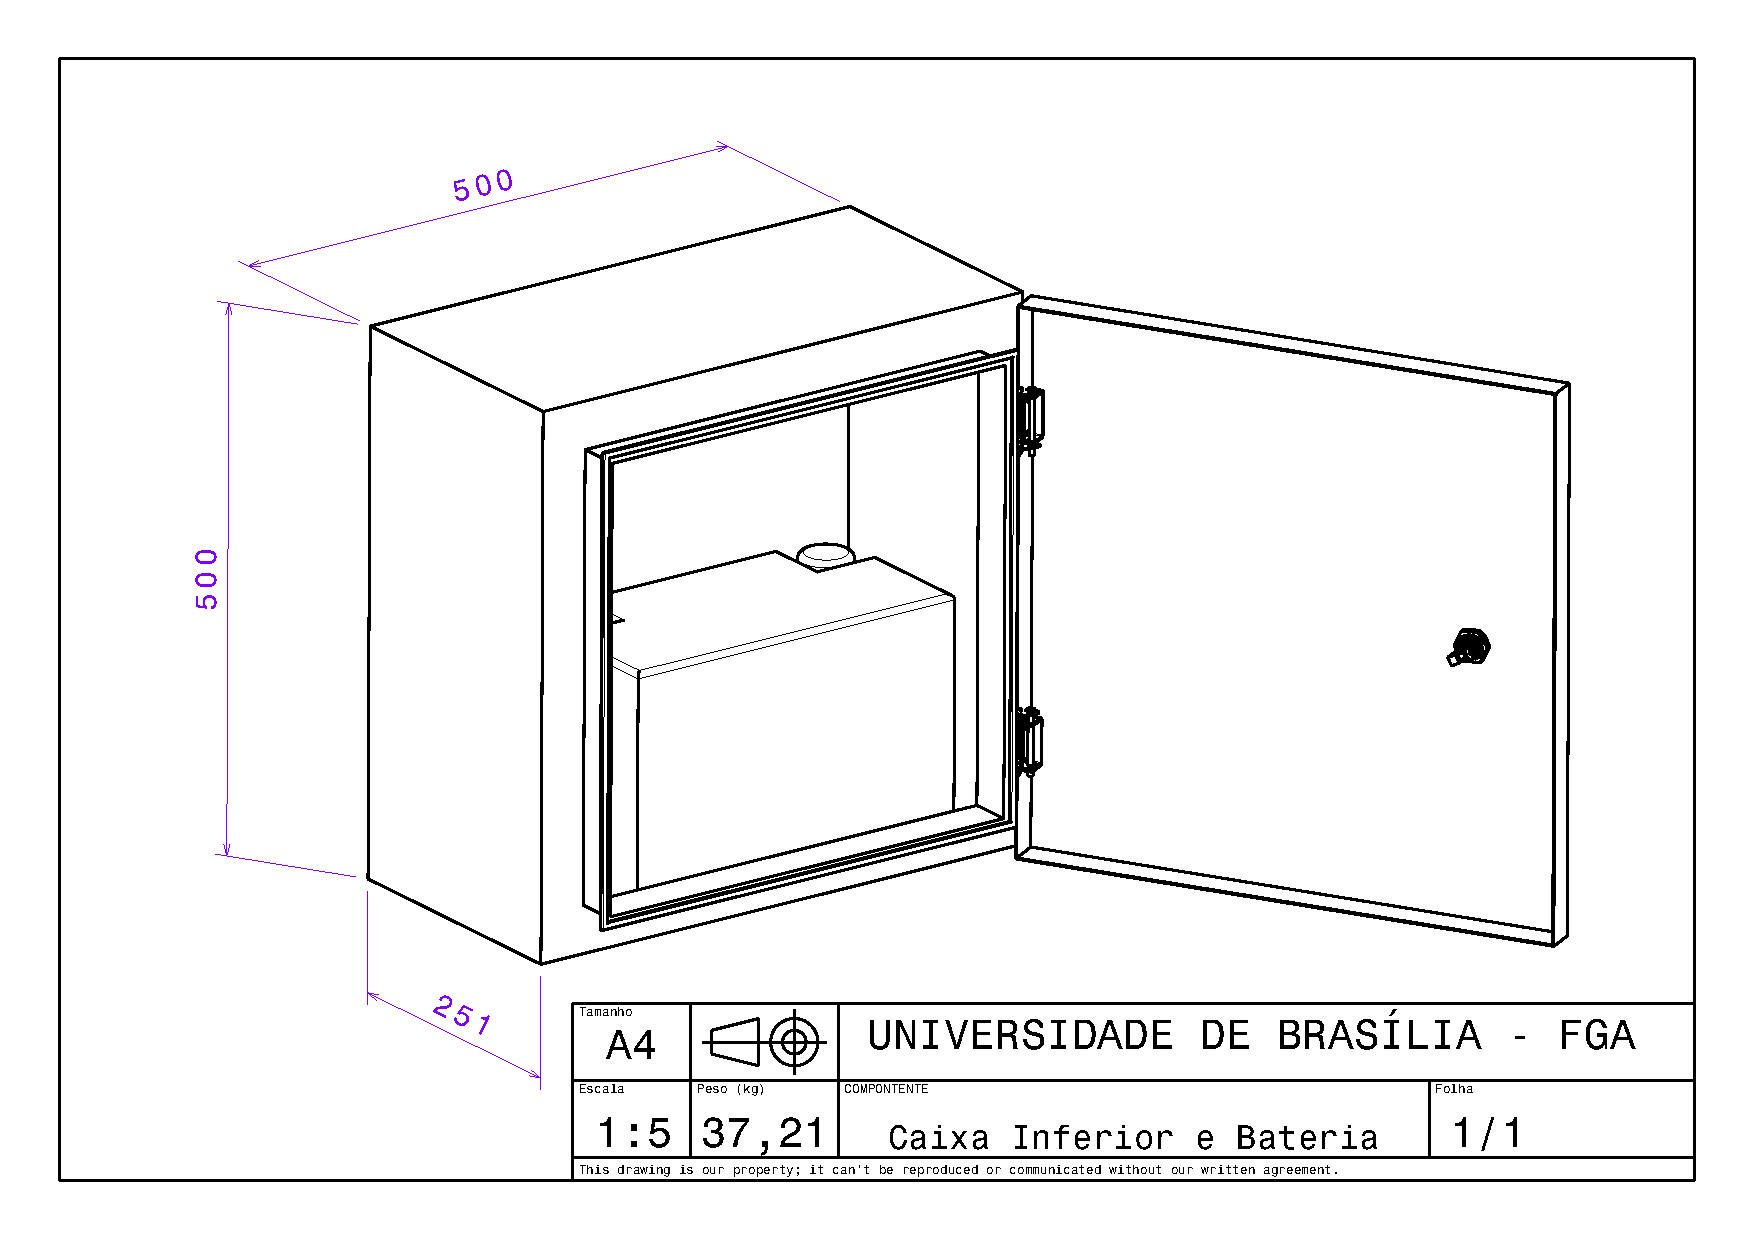
\includepdf[angle=90, scale=0.75]{CaixaInf.pdf}
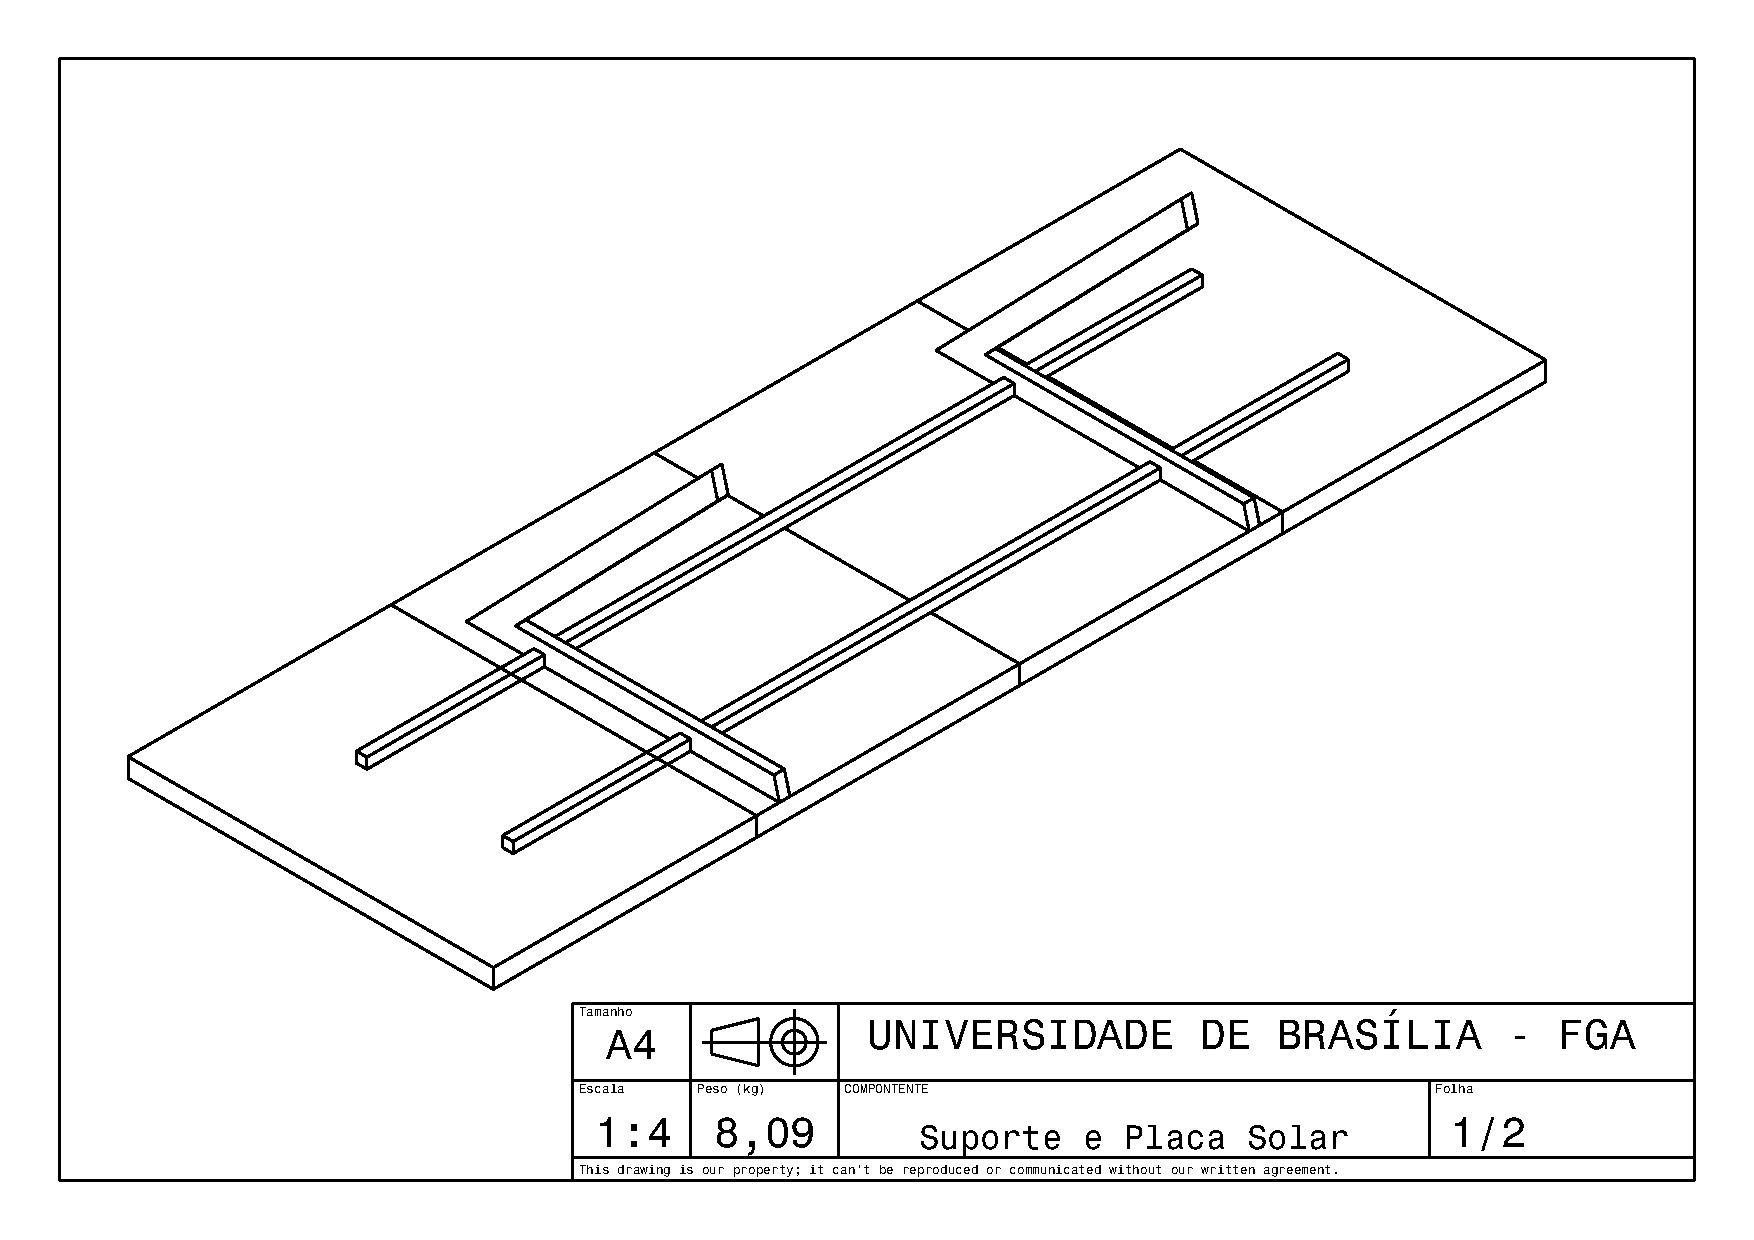
\includepdf[angle=90, scale=0.75]{SuportePainel1.pdf}
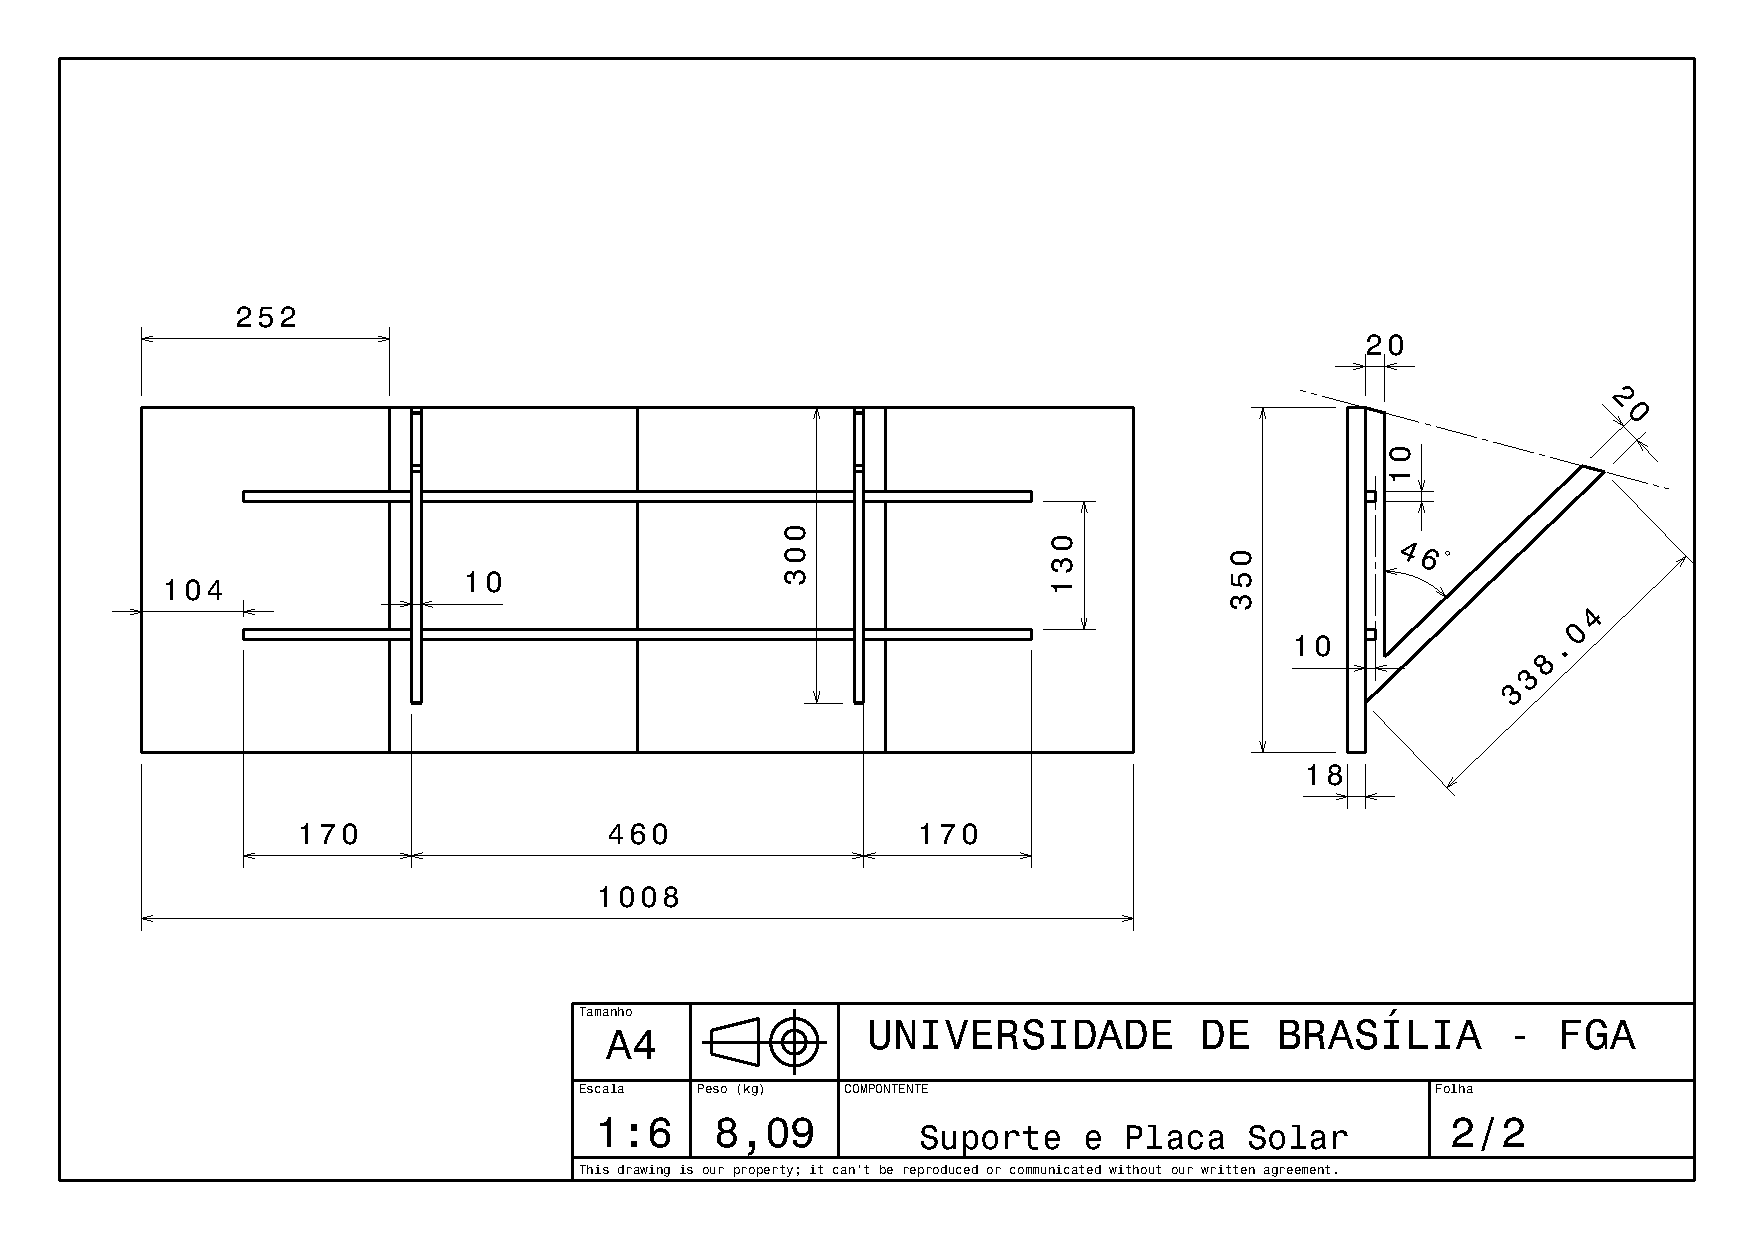
\includepdf[angle=90, scale=0.75]{SuportePainel2.pdf}
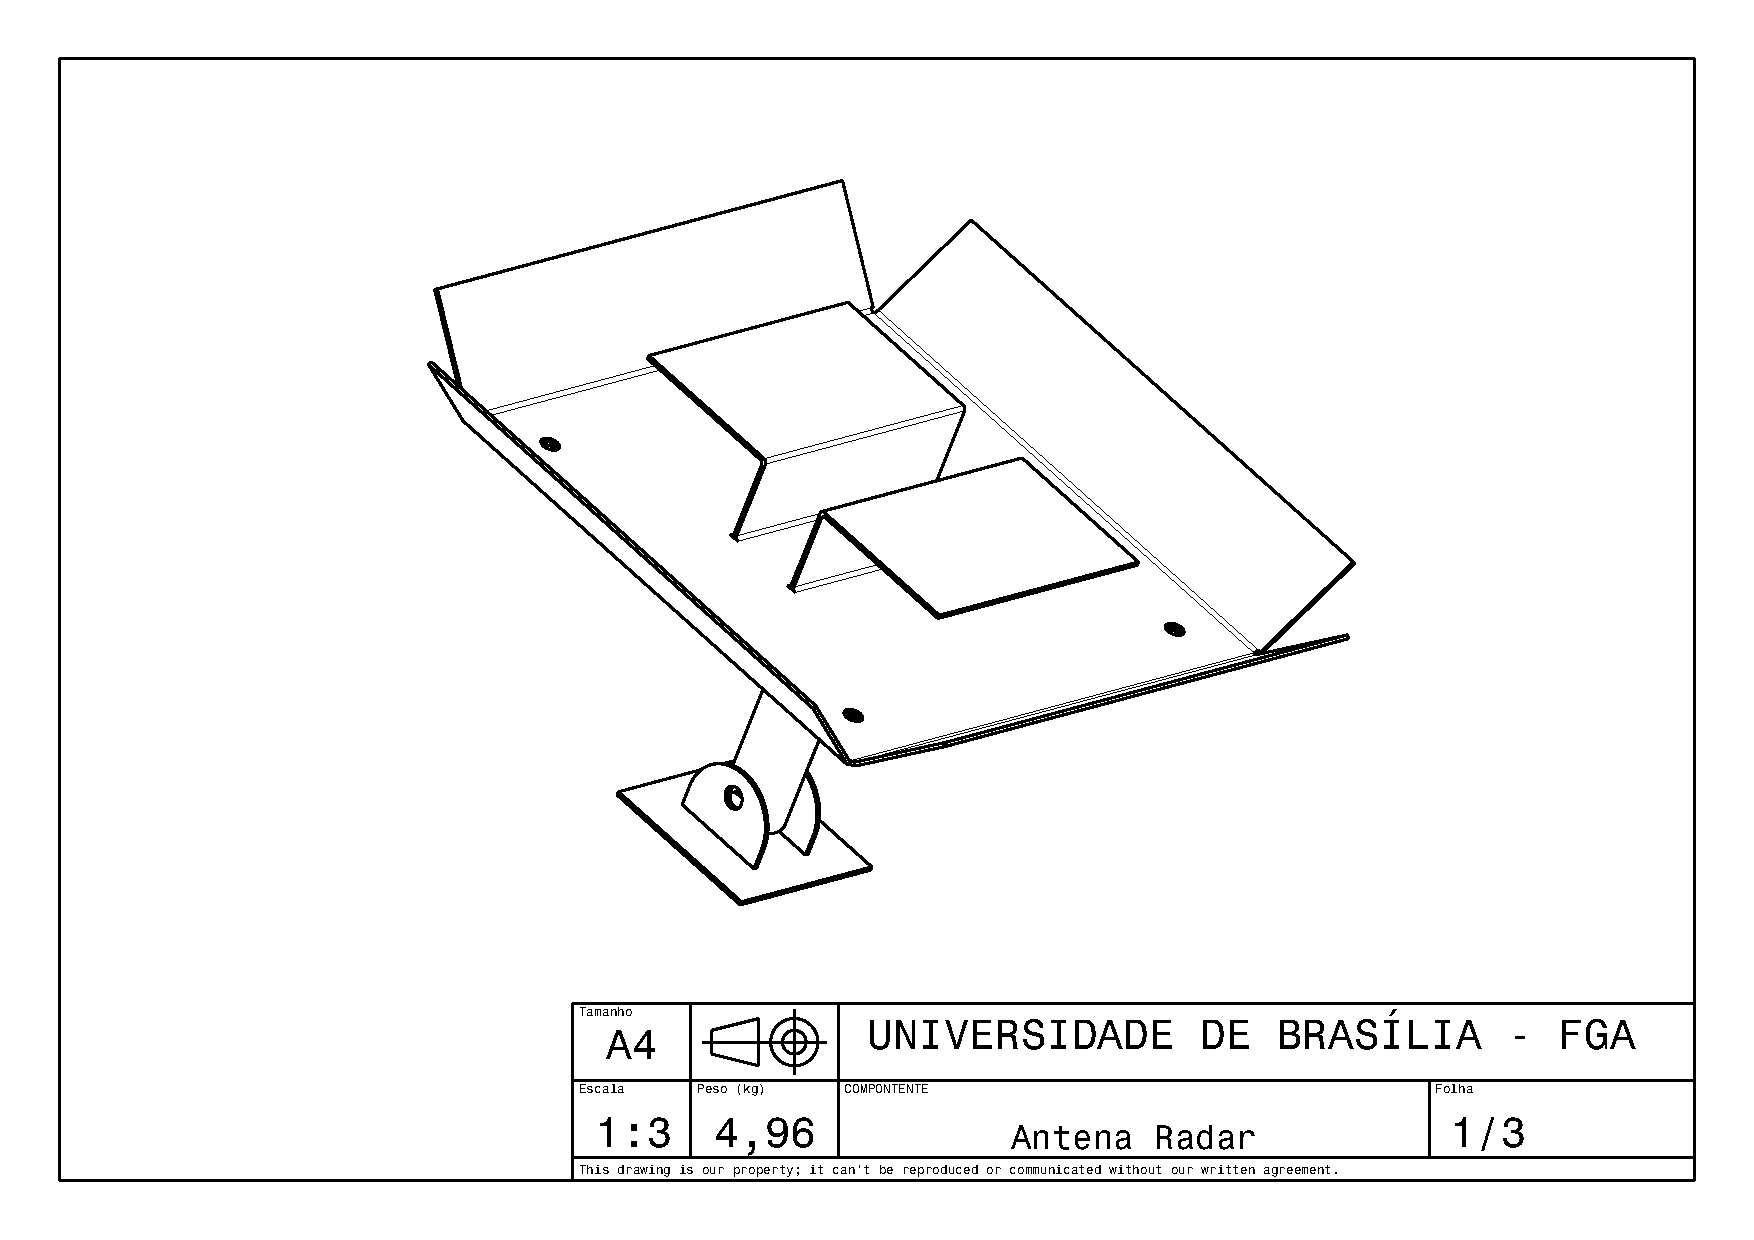
\includepdf[angle=90, scale=0.75]{AntenaRadar1.pdf}
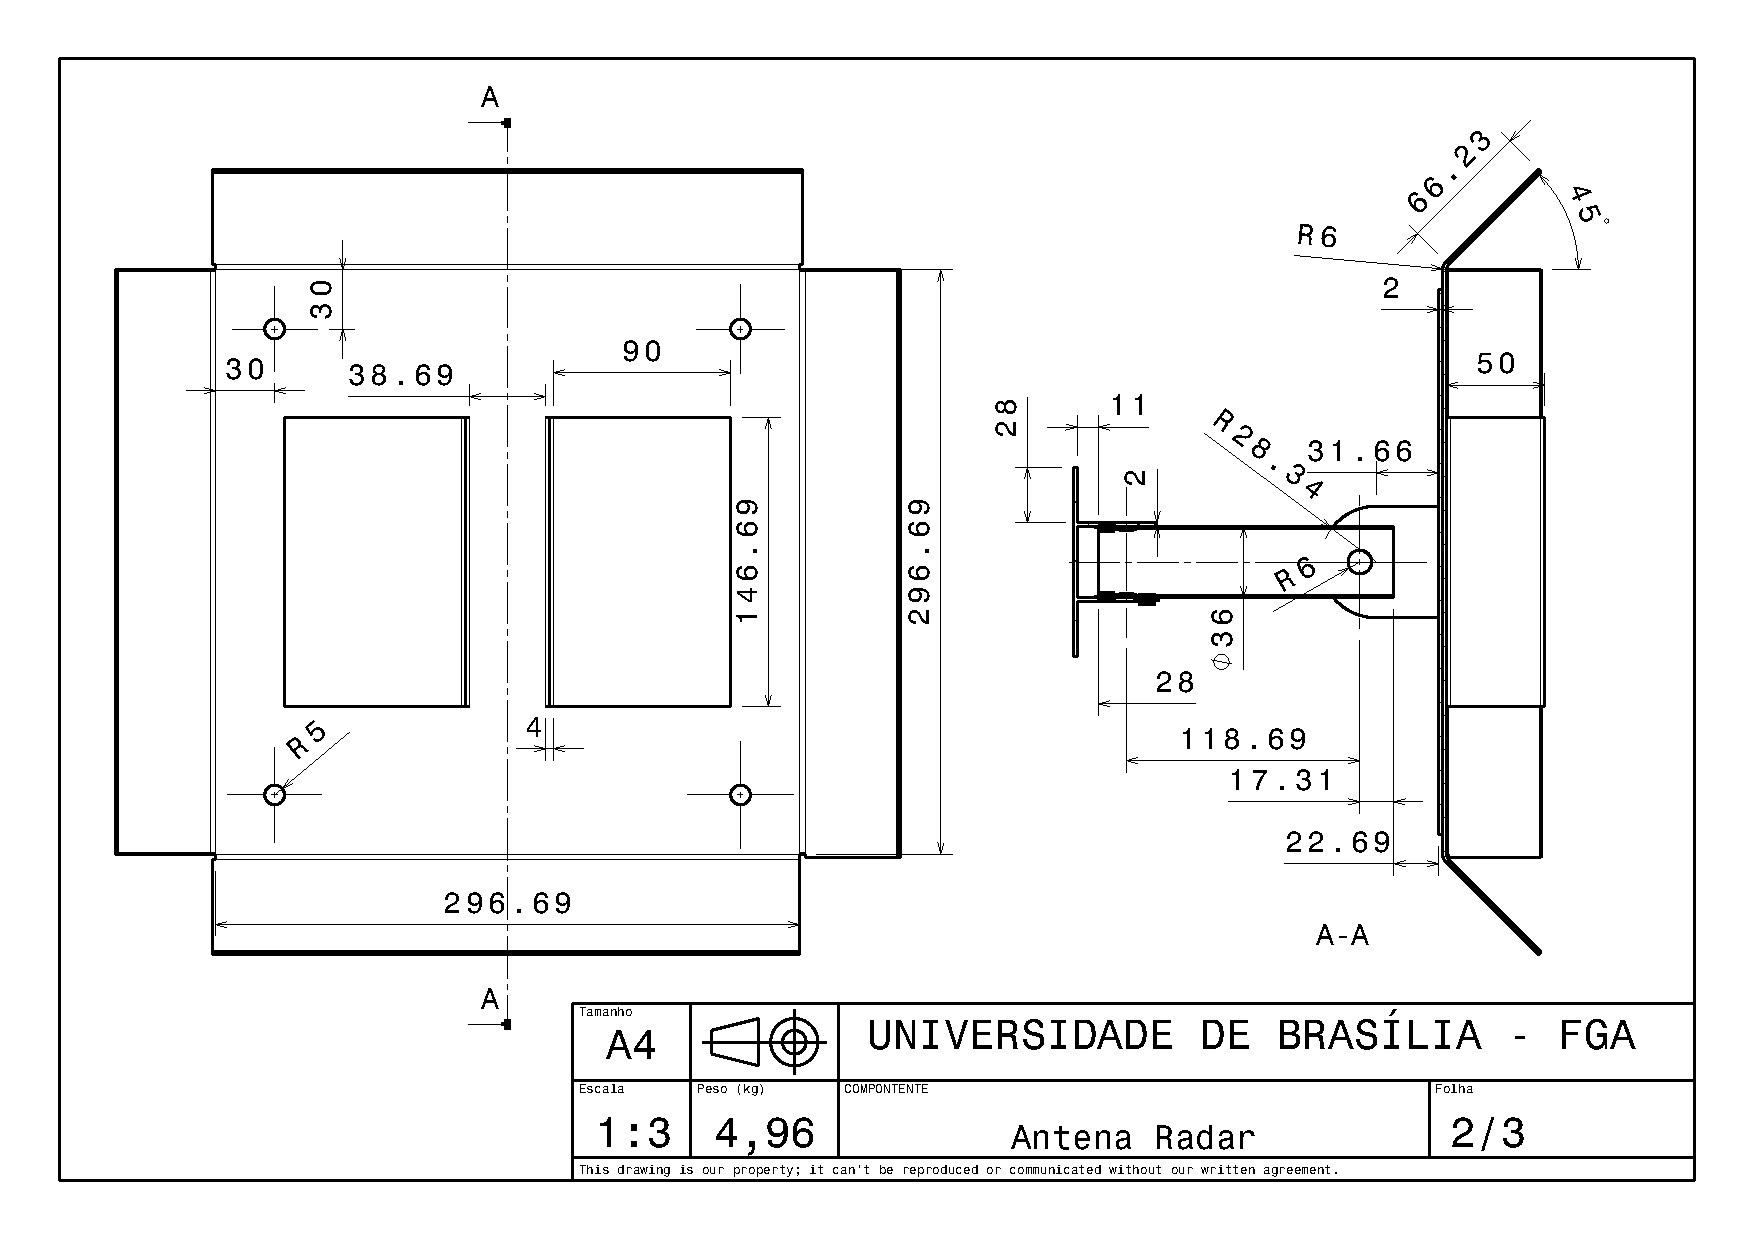
\includepdf[angle=90, scale=0.75]{AntenaRadar2.pdf}
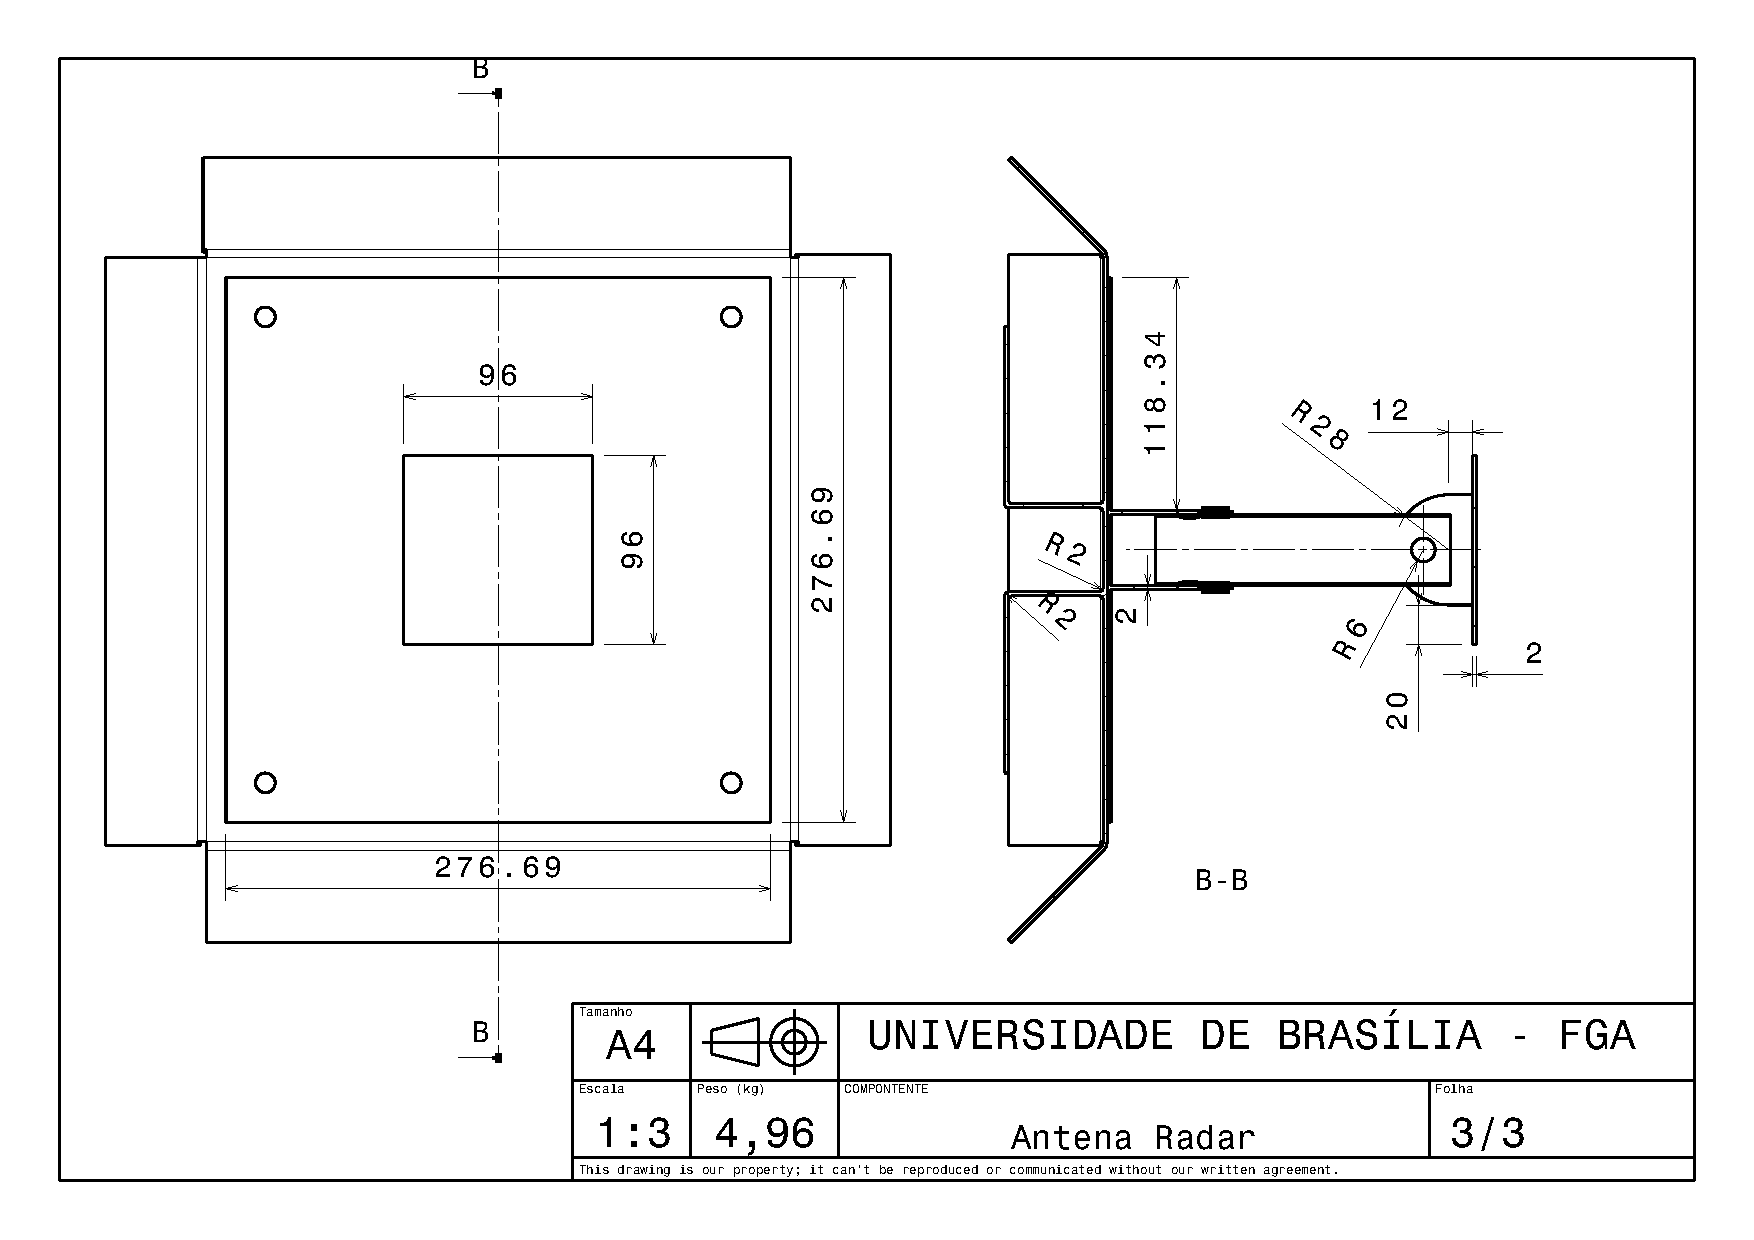
\includepdf[angle=90, scale=0.75]{AntenaRadar3.pdf}
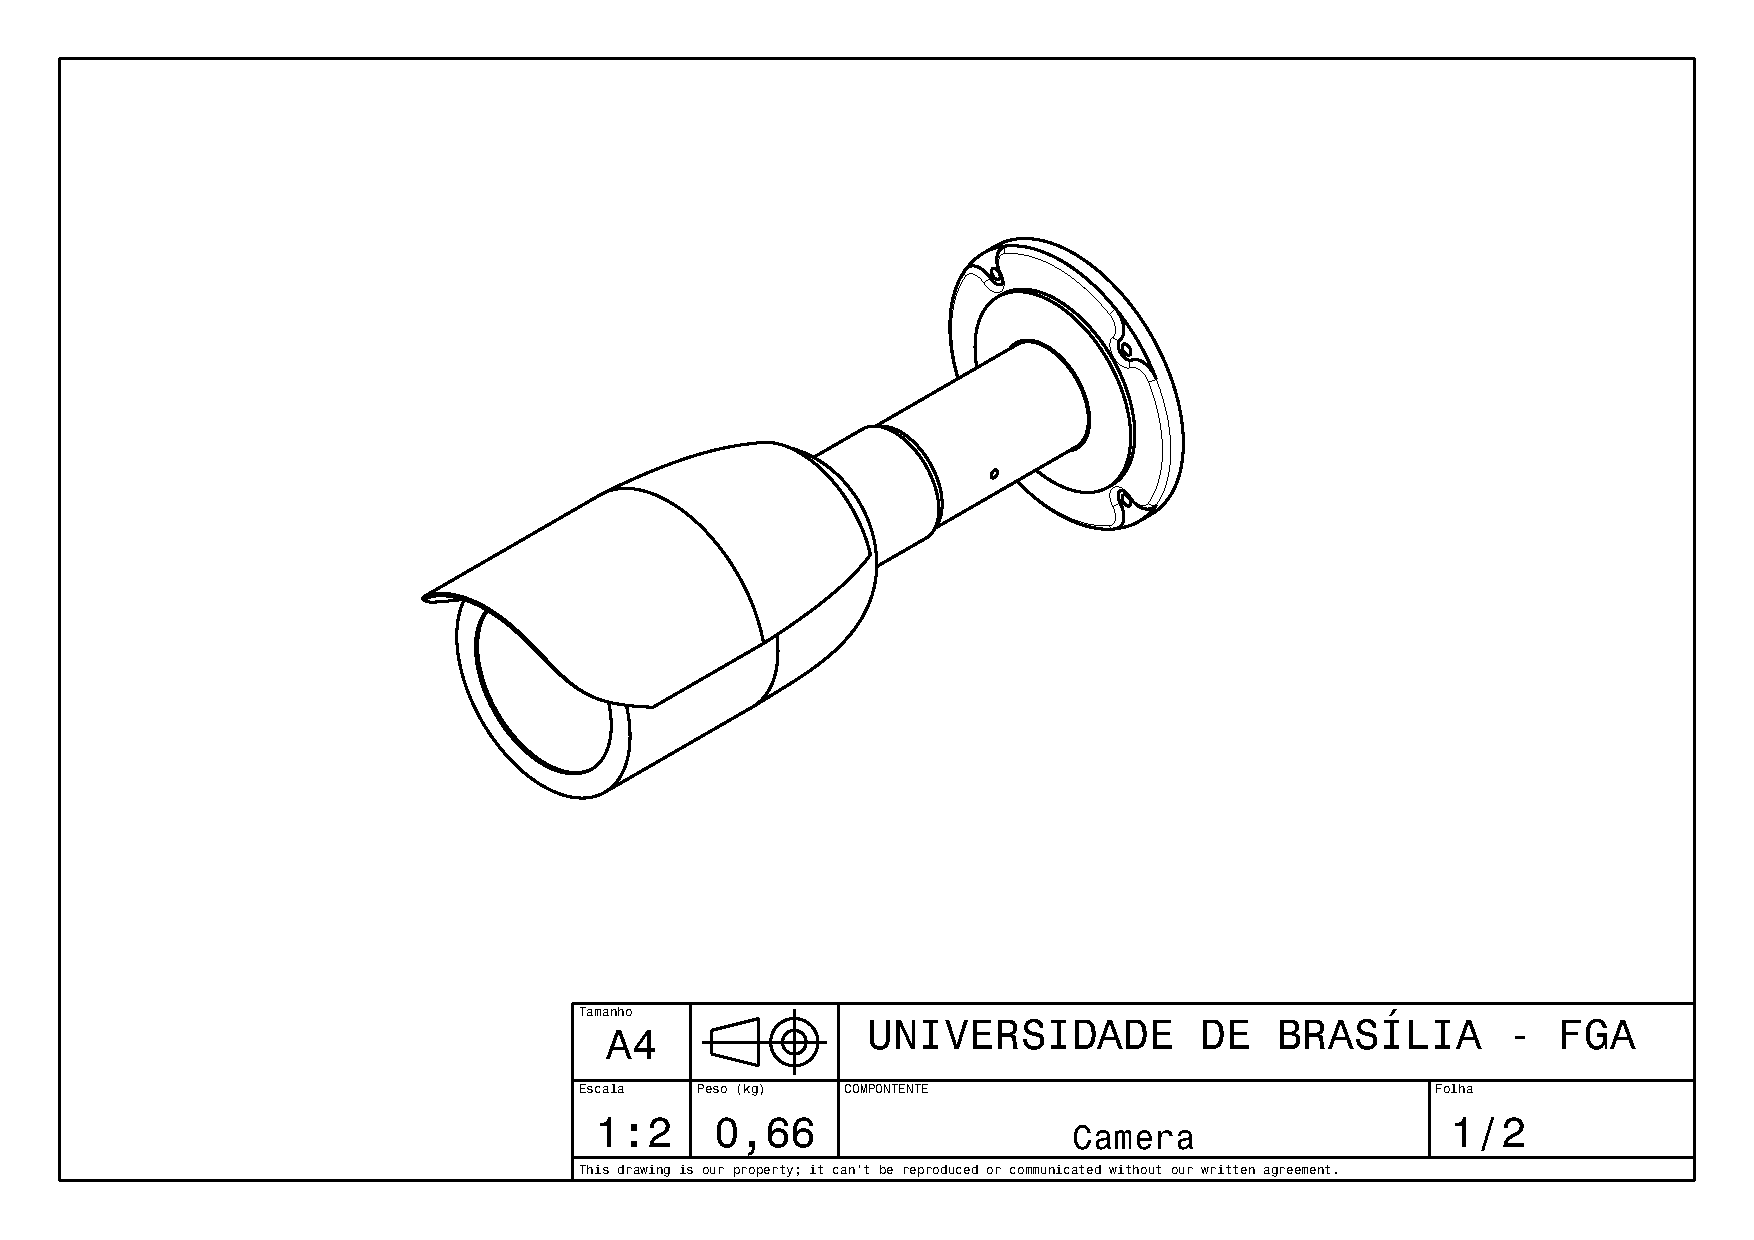
\includepdf[angle=90, scale=0.75]{Camera1.pdf}
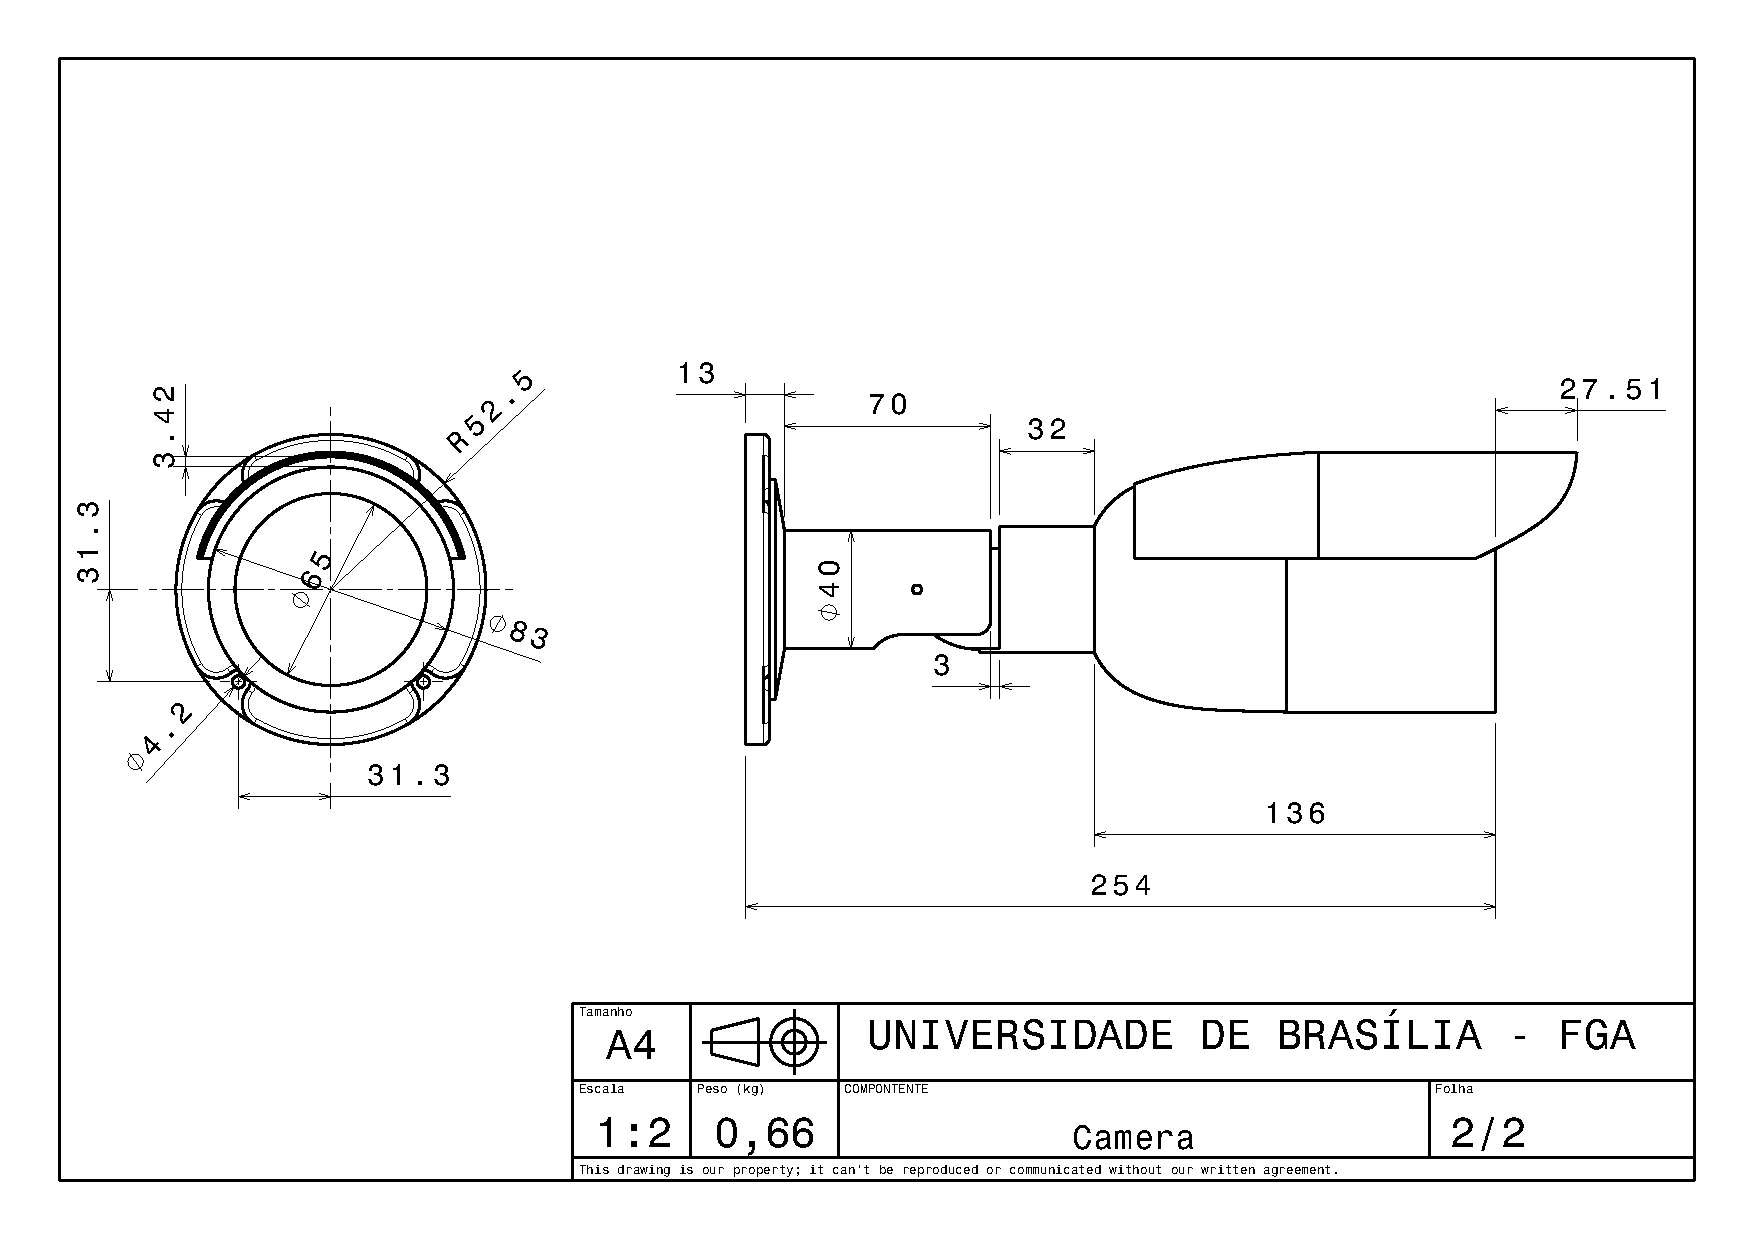
\includepdf[angle=90, scale=0.75]{Camera2.pdf}
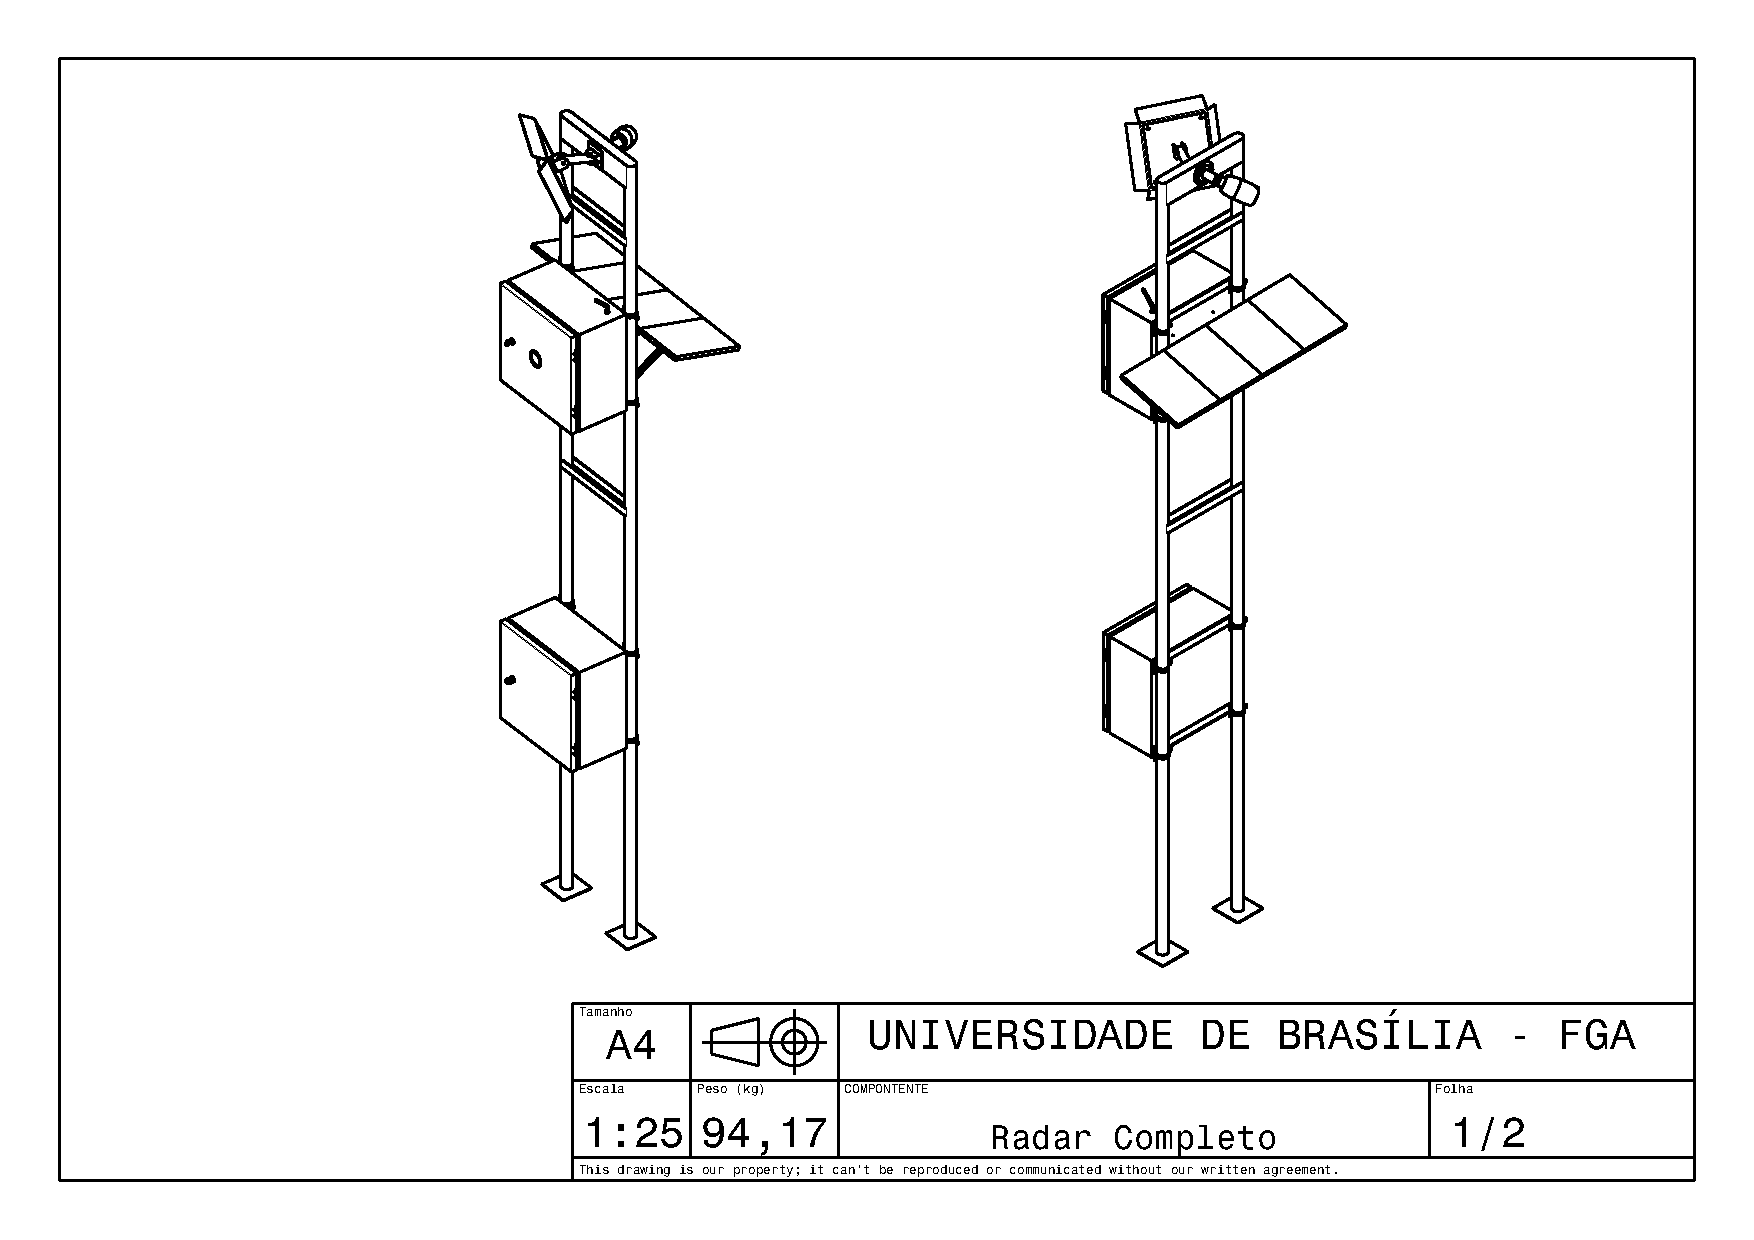
\includepdf[angle=90, scale=0.75]{RadarCompleto1.pdf}
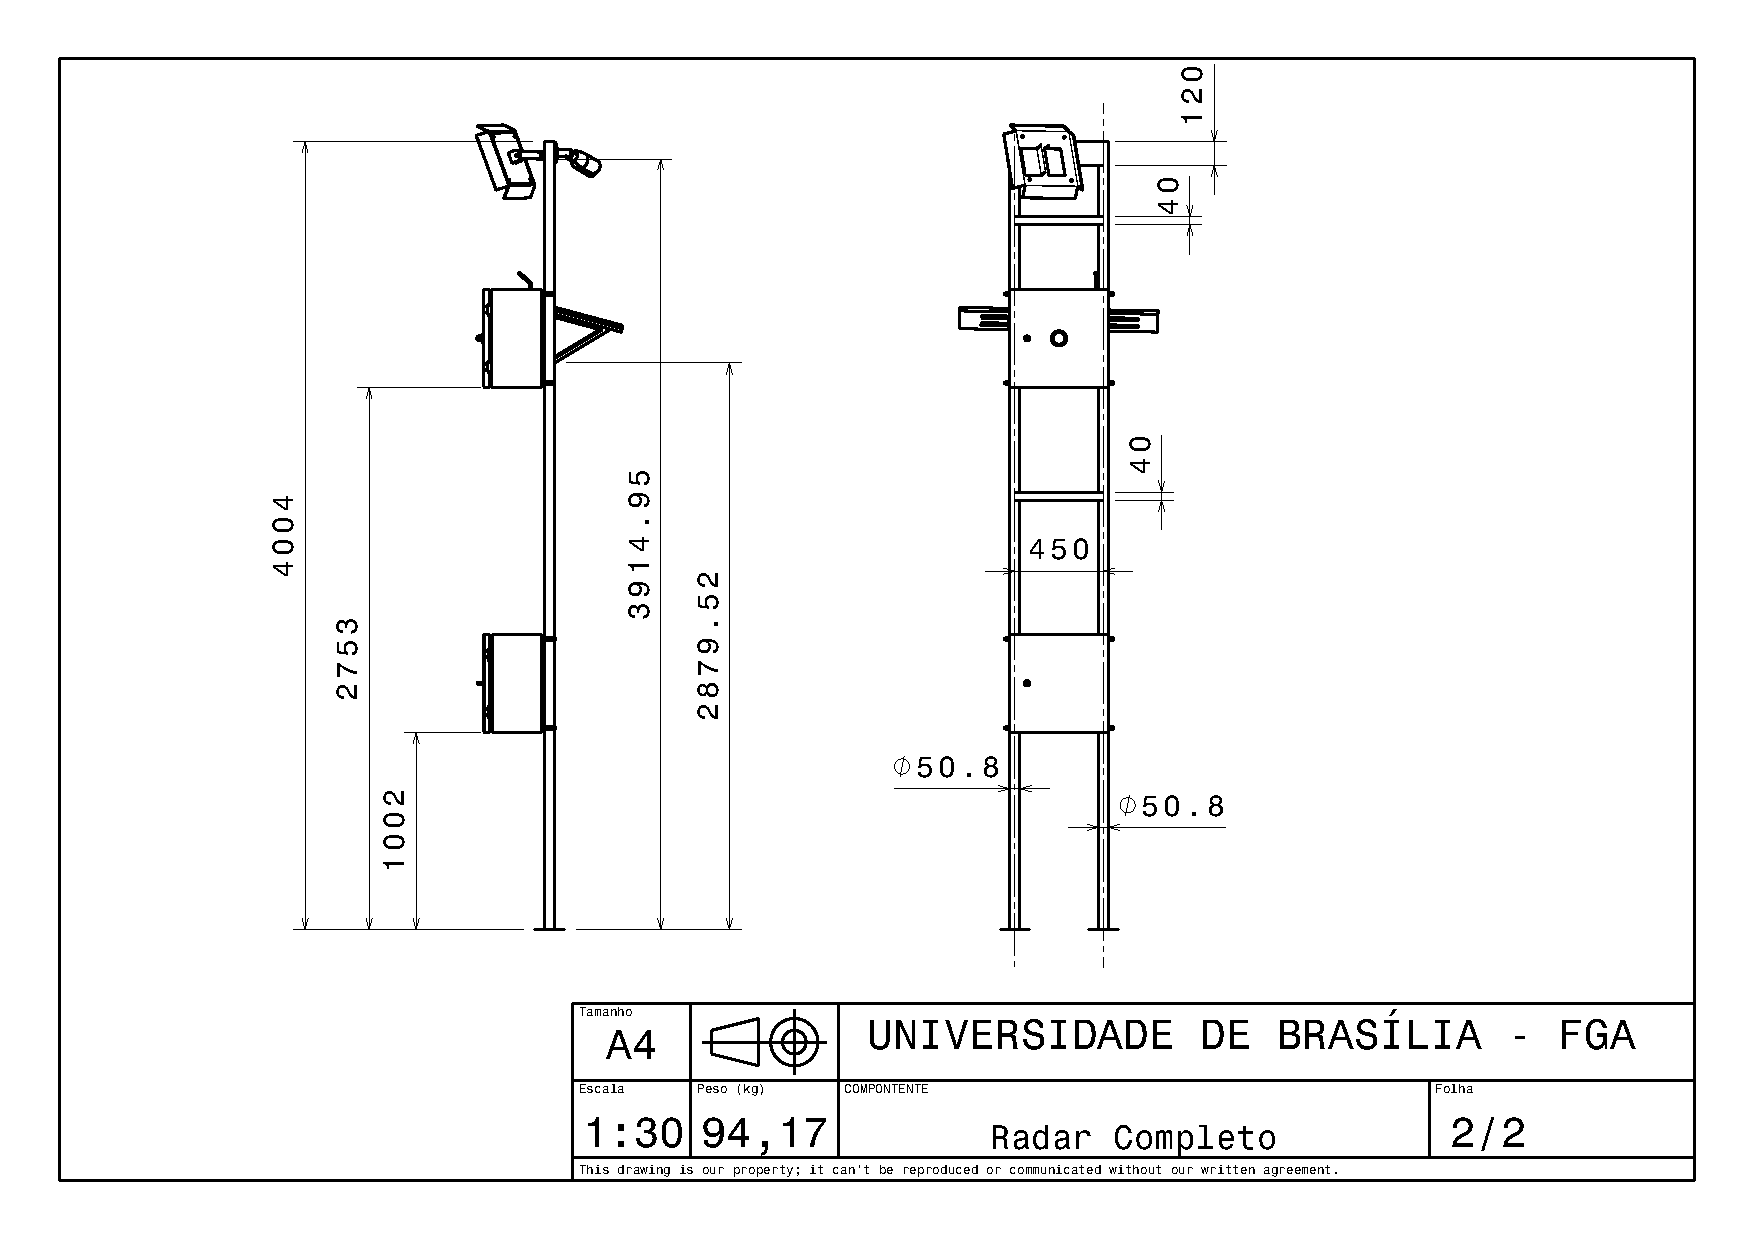
\includepdf[angle=90, scale=0.75]{RadarCompleto2.pdf}

\end{apendicesenv}